\chapter{Modelo implementado e resultados}

O modelo implementado implementa todo o processo através de classes nativas da linguagem Ruby\footnote{http://ruby-lang.org} e de interfaces de comunicação com outros serviços como a Search API do Twitter e a biblioteca LIBSVM.

Para a obtenção das publicações, é utilizada a interface da \textit{Search API} do Twitter para a linguagem. A interface realiza a ponte entre as chamadas HTTP necessárias para a API do Twitter em classes Ruby. Através da interface, são chamados métodos que buscam a palavra-chave ou expressão desejada, entre as datas especificadas. No caso do modelo, a palavra-chave ``manifestação'', entre 01 e 31 de Agosto de 2014. A Search API, porém, não retorna publicações com mais de uma semana de criação\footnote{A interface \textit{Search API} possui a restrição de busca de publicações para apenas uma semana depois da sua criação.}, foi preciso, então, realizar mais de uma busca, em datas diferentes. 

As publicações obtidas são salvas localmente em um arquivo CSV, e posteriormente são separadas em mais dois arquivos, um para a fase de testes e outro para a fase de treino. Para manipular os arquivos, é utilizada a biblioteca \textit{CSV} nativa do Ruby, que permite que sejam criados novos arquivos e carregadas suas informações.

A conversão para o modelo de espaço vetorial é feita utilizando classes para manipulação de cadeias de caracteres (\textit{String}) e vetores (\textit{Array}) do Ruby. Através de métodos dessas classes, é possível aplicar todos os passos da conversão, como: tokenização, pré-processamento, criação do dicionário de termos e conversão para vetores de características.

Com os vetores de características obtidos, a classificação das publicações com SVM é feita utilizando a interface Ruby para biblioteca LIBSVM\footnote{http://www.csie.ntu.edu.tw/~cjlin/libsvm/}. A biblioteca LIBSVM implementa diferentes formulações de máquina de vetores de suporte (SVM) e funções de kernel. A interface para Ruby permite que a biblioteca seja utilizada através de classes da linguagem e que a classificação seja aplicada de forma integrada com o resto do processo.

Após a classificação, é feita a extração dos dados do horário e localização. O horário é extraído diretamente a partir da informação presente no arquivo CSV. A localização, é extraída de acordo com qual dado será utilizado: caso a geolocalização esteja presente, esse dado é diretamente retirado do arquivo. Caso não esteja, é utilizada a informação obtida no processo de tokenização da publicação para identificar se, nos termos presentes, está contida alguma cidade brasileira. Caso no texto não esteja, é aplicada a tokenização na informação do perfil do usuário e realizado o mesmo processo de identificação.

Para a criação do ambiente, foi utilizada a ferramenta para desenvolvimento de aplicações web Ruby on Rails\footnote{http://rubyonrails.org}. No ambiente são exibidos gráficos de série-temporal das publicacões, divididas primeiramente por dias e posteriormente por horas. É possível visualizar cada faixa de horário da publicação em um mapa de marcadores, em que as publicações são agrupadas de acordo com a sua localização, o que permite a visualização do horário e da localização dos eventos. 

O código completo implementado que obtem as publicações, as converte para o modelo de espaço vetorial e a as classifica com SVM, se encontra no Apêndice A. Aqui serão apresentadas apenas as partes mais relevantes do código, de acordo com a organização das seções dos capítulos anteriores.

\section{Obtenção de publicações via Search API}

Para obter as publicações é utilizada a Search API do Twitter, na sua versão 1.1. É utilizada uma interface Ruby para a API, que cria classes para lidar com as chamadas HTTP. Ao invés de lidar com o código referente a requisições HTTP, o que dificulta a sua implementação e legibilidade do código, é possivel lidar direto com métodos de classes Ruby. 

A interface possui o mesmo nome do serviço e o modelo utiliza a sua versão 5.8.0. Para instalar a interface, utitilizamos o gerenciador de extensões do Ruby Rubygems\footnote{https://rubygems.org}. Após a instalação do gerenciador, ela é instalada rodando o código a partir do terminal:

\begin{lstlisting}
  gem install twitter --version 5.8.0
\end{lstlisting}

Com a interface instalada, para realizar chamadas à Search API do Twitter, é preciso cadastrar um \textit{aplicativo} no serviço\footnote{https://apps.twitter.com} e configurar as chaves que são recebidas. São recebidas 4 chaves: uma chave da API (\textit{consumer key}), um código secreto da API (\textit{consumer secret}), um token de acesso do aplicativo (\textit{access token}) e um código secreto do aplicativo (\textit{access token secret}):

\begin{lstlisting}
  class Twitter
    def initialize
      @cliente = Twitter::REST::Client.new do |config|
        config.consumer_key        = "DbT8fYWR2jq1TIXvxVtiZzFno"
        config.consumer_secret     = "3mT9JcwgaWs5gT...tnAWufYMVyUmle"
        config.access_token        = "42659961-4wDJC...gBaE26GpI5kjC3CK"
        config.access_token_secret = "OjhVszJ3Dyivaz...inoaFiWK7FjY"
      end
    end
  end
\end{lstlisting}

Para a configuração no ambiente, é criada a classe Twitter e inicializada a variável para o \textit{@cliente}. A variável recebe uma instância da classe da interface \textit{Twitter::REST::Client}\footnote{em Ruby, ``::'' significa que o termo seguinte é um módulo (ou classe) do anterior} que recebe as chaves criadas em seus respectivos atributos.

Após a configuração das chaves, é possível realizar as chamadas à API. As chamadas são feitas pelo método \textit{Client\#search}\footnote{em Ruby, ``\#'' significa que o termo seguinte é um método de instância do termo anterior}, que recebe como parâmetro a palavra-chave ou expressão à ser buscada e uma instância da classe \textit{Hash} contendo diversas chaves como linguagem, o identificador máximo e mínimo da publicação (retorna apenas publicações com o identificador maior do que o especificado), o limite de publicações a serem retornadas, etc:

\begin{lstlisting}
  publicacoes = @cliente.search("manifestação", lang: "pt", max_id: "200", since_id: "100", count: 100)
\end{lstlisting}

A Search API, porém, exibe duas restrições de busca:

\begin{itemize}
  \item \textbf{Quantidade:} Retorna apenas um número reduzido de publicações por vez.
  \item \textbf{Tempo:} Não retorna publicações mais antigas do que uma semana.
\end{itemize}

Para obter as publicacões em um período de um mês através da Search API, é preciso contornar essas restrições. Para contornar a restrição de quantidade, são criados ciclos de buscas. Para contornar a restrição de tempo, são executados os ciclos em diversas datas diferentes, respeitando os limites de uma semana.

Para determinar o momento de parar o ciclo de buscas, é definida uma data e passada como primeiro parâmetro para o método \textit{Twitter\#buscar}. O segundo parâmetro determina a expressão a ser buscada, e o terceiro o caminho do arquivo CSV que as publicações serão salvas. 

Para cada chamada ao método \textit{Twitter\#buscar}, é executado um ciclo de buscas, tal como mostra as linhas 6 a 10 do código a seguir. Para cada busca, a última publicação retornada tem o seu identificador armazenado, que é passado para a próxima busca, para ser utilizado como o parâmetro \textit{max\_id}. Assim, a cada busca subsequente, apenas as publicações a partir daquele identificador específico são retornadas. Além do \textit{id}, a data da última publicação retornada também é armazenada e, caso seja menor que a passada como parâmetro o ciclo para. O código a seguir representa o primeiro ciclo de buscas:

\begin{lstlisting}
  class Twitter
    def buscar data_limite, expressao, caminho_arquivo
      data_publicacao = Time.now
      id_maximo = nil

      while publication_date > data_limite
        publicacaoes = @cliente.search(expressao, lang: "pt", max_id: id_maximo).to_a
        data_publicacao = publicacaoes.last.created_at
        id_maximo = publicacoes.last[:id] - 1
        (...)
      end
    end
  end
  twitter = Twitter.new
  data_limite = Time.new(2014, 8, 28, 0, 0, 0, "-03:00")
  twitter.buscar data_limite, "manifestação", "publicacoes_0108_0708.csv"
\end{lstlisting}

Para as seguintes datas de busca, a \textit{data\_limite} e o caminho do arquivo (linha 15 e 16 do código anterior) são modificados para que a busca retorne apenas as publicações criadas após a data em que a última busca foi feita, como indicado pelo código a seguir:

\begin{lstlisting}
  data_limite = Time.new(2014, 08, 1, 0, 0, 0, "-03:00")  # No dia 01/08
  twitter.buscar data_limite, "manifestação", "publicacoes_0108_0708.csv"
  data_limite = Time.new(2014, 08, 7, 0, 0, 0, "-03:00") # No dia 07/08
  twitter.buscar data_limite, "manifestação", "publicacoes_0808_1408.csv"
\end{lstlisting}

Para manipular arquivos CSV e salvar as publicações a cada busca, é utilizada a biblioteca do Ruby \textit{CSV}. Para abrir o arquivo é utilizado o método \textit{CSV.open}\footnote{em Ruby, ``.'' significa que o termo seguinte é um método de classe do termo anterior}, que recebe como parâmetros o \textit{nome do arquivo} e o \textit{modo de leitura/gravação}. O modo \textit{a+} é utilizado como modo de gravação, para criar o arquivo para os primeiros resultados da busca e empilhar os resultados das próximas buscas. Outro modos disponíveis \textit{w} para apenas escrita, \textit{r} para apenas leitura, etc\footnote{http://www.ruby-doc.org/core-2.1.2/IO.html}. 

O método \textit{Array\#each} itera entre os elementos do vetor e passa cada elemento para dentro do bloco contido entre \textit{do} e \textit{end}, para que ele possa ser manipulado. A cada iteração, os dados relevantes da publicação são transferidos para a estrutura CSV. O código a seguir apresenta a criação do arquivo de publicações da primeira data de busca:

\begin{lstlisting}
  CSV.open("publicacoes_0108_0708.csv", "a+") do |csv|
    publicacoes.each do |publicacoes| 
      csv << [
        publications[:id], 
        publications.created_at, 
        publications.text, 
        publications.geo.latitude, 
        publications.geo.longitude, 
        publications.user.location
      ]
    end
  end
\end{lstlisting}

Os arquivos de publicações de cada data de busca são unidos manualmente em um único arquivo, que representa o total de publicações obtidas do Twitter, para que as operações futuras possam ser realizadas de modo único. A partir desse arquivo, são gerados mais dois arquivos: um para a fase de treino e um para a fase testes do SVM.

Na fase de treino, para informar as classes das publicacões são adicionadas, ao final de cada linha do arquivo, o valor de sua classe, ``1.0'' para classes positivas e ``-1.0'' para classes negativas. Como o arquivo é separado por vírgulas, basta apenas adicionar, após o último valor de cada linha, uma vírgula separadora e o valor respectivo da classe, gerando a Tabela 5.1:

\begin{table}[ht]
  \caption{Arquivo CSV de teste com suas classes}
  \centering
  \begin{tabular}{| p{1cm} | p{1.7cm} | p{4cm} | p{1.5cm} | p{1.5cm} | p{2cm} | p{1.3cm} | }
    \hline
    \textbf{Id} & \textbf{Horário} & \textbf{Texto} & \textbf{Lat.} &\textbf{Lon.} & \textbf{Localiza. perfil} & \textbf{Classe} \\ [0.5ex] \hline \hline
    49744 40914 21286 400 & 2014-08-07 14:45:23 & Aumento da passagem de ônibus provoca manifestação em sorocaba & -15.850 902 & -47.944 792 & Brazil & 1.0 \\ \hline
    49743 91868 07685 121 & 2014-08-07 14:40:19 & O sorriso é a manifestação dos lábios & -21.167 484 & -41.331 175 & Rio de Janeiro - Brasil & -1.0 \\ \hline
    \hline
  \end{tabular}
  \label{table:nonlin}
\end{table}

Os arquivos são utilizados para realizar a conversão para o modelo de espaço das publicações e, posteriormente, por cada fase da classificação com o SVM.

\section{Conversão para o modelo de espaço vetorial}

Para converter as publicações para o modelo de espaço vetorial, são utilizadas classes nativas da linguagem Ruby para manipulação de cadeias de palavras (\textit{strings}) e vetores. O objetivo da conversão é transformar as publicações do formato de texto para um formato que o classificador SVM consiga tratá-los. A Figura 5.1 ilustra o processo de conversão de uma publicação:

\begin{figure}[htpb]
  \begin{center}
    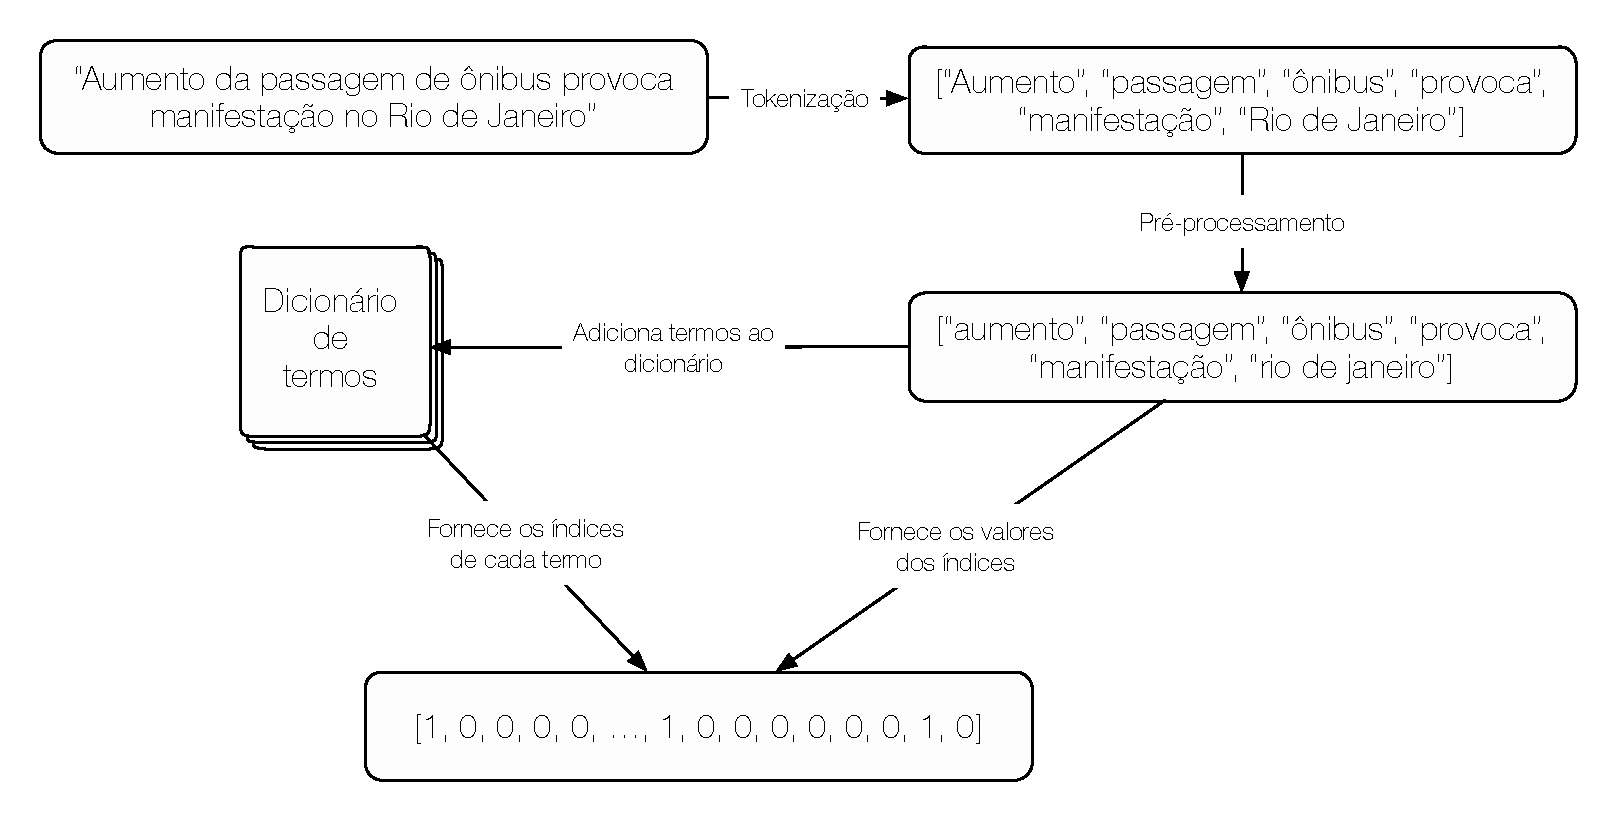
\includegraphics[width=1.0\textwidth]{figuras/conversao-modelo-espaco.eps}
    \caption{Conversão para o modelo de espaço vetorial.}
  \end{center}
\end{figure}

\subsection*{Tokenização e pre-processamento}

Para realizar a \textit{tokenização} dos textos das publicações, é utilizado o método \textit{String\#split}. O método aceita como parâmetro um ou mais caracteres, ou uma expressão regular\footnote{http://turing.com.br/material/regex/introducao.html} para dividir o texto em termos de acordo com esse parâmetro. O texto é quebrado a cada parte que casa com o parâmetro passado. 

O modelo utiliza como parâmetro para o método uma expressão regular separa os termos da publicação, primeiramente, de acordo com a lista de cidades do Brasil, e posteriormente por espaços, como está indicado no código a seguir. Se uma cidade é encontrada na publicação, é gerado apenas um termo, por exemplo, ``Rio de Janeiro'' gera apenas um termo.

\begin{lstlisting}
  /(\bCidade 1\b)|(\bCidade 2\b)|...|(\bCidade N-1\b)|(\bCidade N\b)|\s/
\end{lstlisting}

Na expressão regular, encontram-se os seguintes operadores:

\begin{itemize}
  \item \textbf{``$\mid$''}: captura uma expressão ou outra.
  \item \textbf{``\textbackslash s''}: captura espaços
  \item \textbf{``\textbackslash b''}: captura quebra de expressão como espaço, início ou fim de linha
  \item \textbf{``('' e ``)''}: identificador para retornar a expressão neles contida
\end{itemize}

Ao pedir para o método dividir a expressão a partir dessa expressão regular, está se dizendo para dividir a expressão pela ``Cidade 1'' ou a ``Cidade 2'' ou a ``Cidade 3'', e assim por diante até a ``Cidade N'', ou por espaço, ao final. O resultado da divisão de termos para a publicação ``Manifestação hoje no Rio de Janeiro'' será:

\begin{lstlisting}
  expressao = "Manifestação hoje no Rio de Janeiro"
  expressao.split(/(Rio de Janeiro)|(São Paulo)\s/)
  # => ["Manifestação", "hoje", "no", "Rio de Janeiro"]
\end{lstlisting}

Para criar os termos das cidades do Brasil, é utilizada uma lista de cidades\footnote{http://samus.com.br/web/site/artigo-todas\_as\_cidades\_do\_brasil\_atualizado\_e\_com\_acentos}, que é salva em uma estrutura JSON em que as chaves são as cidades e os valores são os estados, para posteriormente mapear as cidades aos estados. O processo de conversão do JSON para a expressão regular está identificado Figura 5.2.

\begin{figure}[htpb]
  \begin{center}
    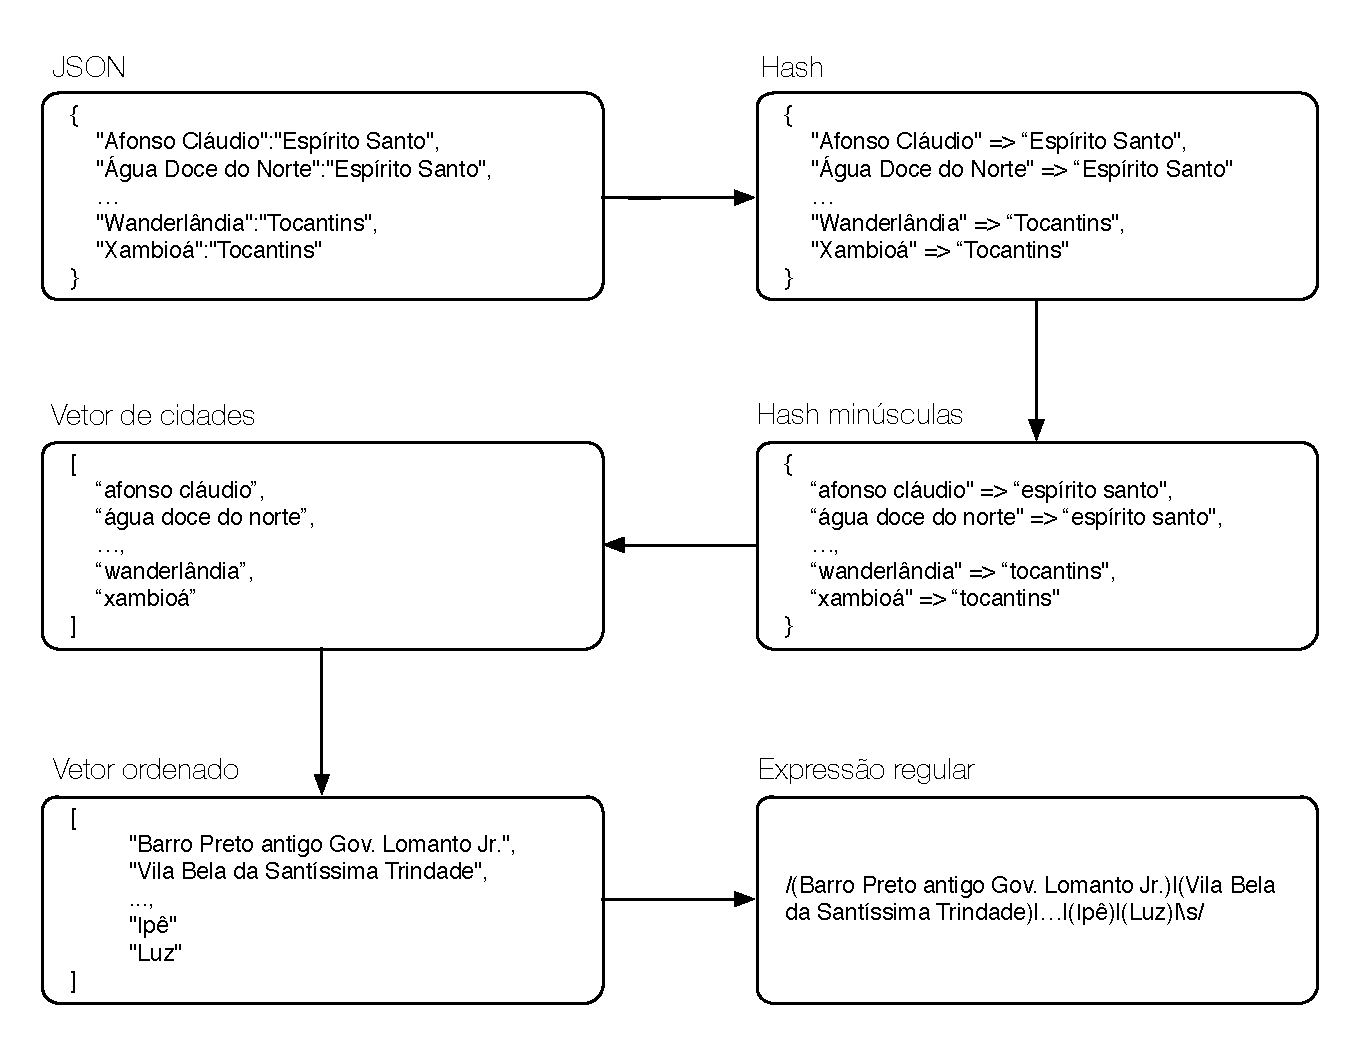
\includegraphics[width=0.9\textwidth]{figuras/criacao-regexp.eps}
    \caption{Criação da expressão regular.}
  \end{center}
\end{figure}

Para converter as cidades da estrutura JSON para \textit{Hash}, são utilizados os métodos \textit{IO.read}, que se encarrega de ler o arquivo, e \textit{JSON.parse}, que trata de convertê-lo, como indicado na linha 2 do código a seguir. A seguir, todas as chaves e valores do \textit{Hash} são iterados pelo método \textit{Hash\#each\_with\_object} para convertê-los para minúsculas, como indicado nas linha 3, 4 e 5. Para retirar as cidades, é utilizado o método \textit{Hash\#keys}, como indicado na linha 6 do código a seguir:

\begin{lstlisting}
  class String
    JSON_CIDADES = JSON.parse(IO.read("support/cidades_do_brasil.json"))
    ESTADOS_E_CIDADES = JSON_CIDADES.each_with_object({}) do |(k,v), h|
      h[k.downcase] = v.downcase
    end
    LISTA_DE_CIDADES = ESTADOS_E_CIDADES.keys.sort_by { |c| c.length }.reverse
    (...)
  end
\end{lstlisting}

A lista de cidades é ordenada da cidade com o maior nome para a menor, pois a ordem das cidades na expressão regular influencia no modo de criação dos termos a partir do texto da publicação. Isso é preciso ser feito, para que cidades como ``Porto Alegre'' sejam identificadas corretamente, sendo que a cidade ``Porto'' também existe. Caso contrário, a expressão iria identificar o termo ``Porto'' da cidade ``Porto Alegre'' como sendo uma cidade separada, ao invés de identificar que o mesmo termo está junto com o termo ``Alegre'', o que o caracteriza como uma outra cidade.

Para ordená-los dessa maneira, é utilizado o método \textit{Array\#sort\_by}, passando o tamanho de cada termo dentro do bloco, e a seguir é aplicado o método \textit{Array\#reverse} para reordená-los do maior para o menor, como indicado na linha 6 do código anterior.

A seguir as cidades são unidas através da iteração do vetor e na substituição de cada termo por seu constituinte dentro da expressão regular: ``Rio de Janeiro'' se torna ``\b(Rio de Janeiro)\b''. Os termos são então unidos em uma única cadeia de caracteres através do método \textit{Array\#join}, passando como parâmetro o operador ``ou'' da expressão regular, como indicado na linha 3 do código a seguir. Por fim, na linha 4, é criada a expressão regular a partir das cidades unidas, com o final da expressão indicando ``ou espaço'':

\begin{lstlisting}
  class String
    # (...)
    CIDADES_UNIDAS = LISTA_DE_CIDADES.map { |city| "(\\b#{city}\\b)" }.join("\|")
    CIDADES_EXPREG = Regexp.new "#{CIDADES_UNIDAS}|\\s"
  end
\end{lstlisting}

Após a conversão dos termos, os mesmos tem todos os caracteres de pontuação retirados utilizando o método \textit{String\#gsub}. O método recebe dois parâmetros: o primeiro é o trecho que se deseja substituir, e o segundo o trecho para qual irá substituí-lo. No primeiro parâmetro é passada uma expressão regular que representa todos os caracteres de pontuação. No segundo, não é passado caractere nenhum, o que indica que se deseja remover os trechos passados no primeiro parâmetro, como indicado na linha 3 do código a seguir.

Alguns termos também são ignorados, como preposições e pronomes. Os termos que são ignorados são identificados a partir de um vetor de exceções. Para deletar os respectivos termos do vetor de termos, é utilizado o método \textit{Array\#delete\_if}, que recebe um bloco e deleta o elemento do vetor caso o resultado operação lógica dentro do bloco retorne verdadeiro, como indicado na linha 4 do código a seguir.

A expressão lógica utilizada para determinar se o termo é deletado ou não, inclui a verificação se o termo se encontra no vetor de exceções, através do método \textit{Array\#include?}, e também da verificação se o termo possui sequências de caracteres como ``http://'' ou ``kk'' ou ``haha'', através do método \textit{String\#include?}, como indicado nas linhas 5 e 6 do código a seguir:

\begin{lstlisting}
  class String
    def tokenizar
      termos = self.downcase.split(CIDADES_EXPREG).map! { |termo| termo.gsub(/\p{^Alnum}\s/, '') }
      termos.delete_if do |termo| 
        termo == "" || EXCECOES.include?(termo) || termo.include?("http") || 
        termo.include?("@") || termo.include?("kk") || termo.include?("haha")
      end
    end
  end
\end{lstlisting}

\subsection*{Dicionário de termos e vetor de características}

O dicionário de termos é criado à partir do conjunto de termos de todas as publicações. Os termos de todas as publicações são recolhidos, como indica as linhas 4 e 5 do código, e são utilizados os métodos \textit{Array\#flatten}, \textit{Array\#uniq} e \textit{Array\#sort} para criar o dicionário, como indica a linha 6 do código:

\begin{lstlisting}
  class Treinador
    #(...)
    def criar_dicionario_de_termos
      @dicionario_de_termos = @publicacoes_de_treino.map do |publicacao| 
        publicacao.termos
      end.flatten.uniq.sort
    end
    #(...)
  end
\end{lstlisting}

O método \textit{Array\#flatten} é utilizado para reduzir vetores à apenas uma dimensão. Ele é necessário pois as publicações encontram-se cada uma em um vetor de termos, sendo a lista de todas uma matriz de termos. \textit{Array\#uniq} é utilizado para reduzir os termos à apenas uma ocorrência de cada um, e \textit{Array\#sort} para ordenar os termos por ordem alfabética.

Com o dicionário construído, o vetor de características de cada publicação é obtido através da iteração entre os termos do dicionário e a atribuição do valor ``1'' caso os termos da publicação incluam o respectivo termo do dicionário, e ``0'' caso não incluam, como indica a linha 5 do código a seguir. Posteriormente, é preciso converter o vetor para a estrutura interna do LIBSVM, como está na linha 7 do código:

\begin{lstlisting}
  class Publicacao
    # (...)
    def vetor
      vetor = @treinador.dicionario_de_termos.map do |termo| 
        @termos.include?(termo) ? 1 : 0
      end
      Libsvm::Node.features(vetor)
    end
    # (...)
  end
\end{lstlisting}

\subsection*{Extração}

Para obter a cidade e o estado da publicação é identificado, primeiramente, se os termos da informação da localização do usuário incluem alguma cidade da lista de cidades previamente criadas. Para isso, é aplicada a tokenização na informação da localização e utizado o método \textit{Array\#include?} para verificar se a lista de cidades inclui o termo da localização. Caso localização definida pelo usuário não inclua cidade alguma, é verificado através do mesmo método se a publicação inclui alguma cidade, como indicado no código a seguir:

\begin{lstlisting}
  class Publicacao
    def initialize
      # (...)
      @cidade = extrair_cidade
    end

    def extrair_cidade
      cidade = ""
      if @localizacao_no_perfil
        @localizacao_no_perfil.tokenizar.each do |termo|
          if String::LISTA_DE_CIDADES.include?(termo)
            cidade = termo
          end
        end
      end
      if cidade == ""
        @termos.each do |termo|
          if String::LISTA_DE_CIDADES.include?(termo)
            cidade = termo
          end
        end
      end
      cidade
    end
    # (...)
  end
\end{lstlisting}

\section{Classificação com SVM}

A classificação das publicações é feita uiltizando a interface Ruby da biblioteca LIBSVM ``rb-libsvm''\footnote{https://github.com/febeling/rb-libsvm}, na versão 1.1.5. A interface permite manipular a biblioteca a partir de classes e métodos Ruby. A LIBSVM implementa uma variedade SVMs, regressão de vetores de suporte (SVR) e classificação de vetores de suporte (SVC), é compatível com SVMs de duas ou mais classes e disponibiliza diversas funções de kernel para a sua utilização, possuindo implementações nas linguagens C++ e Java e interfaces para Ruby, Python, PHP, MATLAB, etc.

A interface ``rb-libsvm'' já inclui a biblioteca LIBSVM, eliminando a necessidade da instalação de qualquer outro programa. Para configurar o ambiente para a classificação com o uso de SVM em Ruby, roda-se o seguinte código a partir do terminal:

\begin{lstlisting}
  gem install rb-libsvm --version 1.1.5
\end{lstlisting}

\subsection*{Treinamento}

Para o treinamento do SVM, são utilizadas as classes criadas pela interface com o LIBSVM, são elas: \textit{Libsvm::Problem} e \textit{Libsvm::Parameter}.

A classe \textit{Libsvm::Problem} é encarregada de receber o conjunto de $n$ descritores $({x}_{i}, {y}_{i})$, compostos pelos vetores de características ${x}_{i}$ e a suas respectivas classes ${y}_{i}$, como por exemplo da forma da Tabela 5.2:

\begin{table}[ht]
  \caption{Conjunto de descritores}
  \centering
  \begin{tabular}{| c | c | c |}
    \hline
    \textbf{Sejam} & \textbf{${x}_{i}$} & \textbf{${y}_{i}$} \\ [0.5ex] \hline \hline
    1 & [1, 0, 0, 1, 0, 0, ..., 0, 0, 1] & 1.0 \\ \hline
    2 & [0, 0, 0, 1, 1, 0, ..., 0, 1, 0] & 1.0 \\ \hline
    3 & [0, 1, 0, 1, 0, 0, ..., 0, 0, 0] & -1.0 \\ \hline
    ... & ... & ... \\ \hline
    n-1 & [0, 0, 1, 0, 0, 0, ..., 1, 0, 1] & -1.0 \\ \hline
    n & [1, 0, 0, 0, 0, 0, ..., 1, 1, 1] & 1.0 \\ \hline
    \hline
  \end{tabular}
  \label{table:nonlin}
\end{table}

\begin{table}[ht]
  \caption{Conjunto de descritores}
  \centering
  \begin{tabular}{| c |}
    \hline
    \textbf{${x}_{i}$} \\ [0.5ex] \hline \hline
    [1, 0, 0, 1, 0, 0, ..., 0, 0, 1] \\ \hline
    [0, 0, 0, 1, 1, 0, ..., 0, 1, 0] \\ \hline
    [0, 1, 0, 1, 0, 0, ..., 0, 0, 0] \\ \hline
    ... \\ \hline
    [0, 0, 1, 0, 0, 0, ..., 1, 0, 1] \\ \hline
    [1, 0, 0, 0, 0, 0, ..., 1, 1, 1] \\ \hline
    \hline
  \end{tabular}
  \label{table:nonlin}
\end{table}

A classe \textit{Libsvm::Parameter} encapsula os ajustes dos parâmetros do SVM. Para o modelo implementado, apenas o parâmetro de custo ($C$) (indicado na Equação 4.1) é ajustado, porém também é necessário inicializar os valores dos parâmetros \textit{epsilon} e \textit{cache size}, porém seus valores não são alterados da sua configuração inicial. O código a seguir apresenta a inicialização das classes do LIBSVM e dos parâmetros:

\begin{lstlisting}
  class Classificador
    # (...)
    def initialize
      # (...)
      @problema = Libsvm::Problem.new
      @parametro = Libsvm::SvmParameter.new
      inicializa_parametros
    end

    def inicializa_parametros
      @parametro.cache_size = 1
      @parametro.eps = 0.001
      @parametro.c = 0.1 # cost
    end
    # (...)
  end
\end{lstlisting}

Para carregar as publicações de treino, as publicação são lidas a partir do arquivo CSV e é instanciada uma classe \textit{Publicação} para cada linha do arquivo:

\begin{lstlisting}[caption=Carregamento de publicações]
  class Treinador
    # (...)
    def carregar_publicacoes_de_treino caminho
      CSV.open(caminho) do |csv|
        csv.each do |linha|
          @publicacoes_de_treino << Publicacao.new(linha, self)
        end
      end
    end
    # (...)
  end
\end{lstlisting}

Como o processo de extração do vetor de características de cada publicação já está definido, basta obter agora as suas classes, que estão contidas na posição 6 de cada linha do arquivo CSV. Para obtê-las, então, basta iterar entre as publicações e guardar a posição 6 de cada uma, como indicado na linha 4 do código a seguir:

\begin{lstlisting}
  class Treinador
    # (...)
    def classes
      @publicacoes_de_treino.map { |publicacao| publicacao.linha_csv[6].to_i }
    end
    # (...)
  end
end
\end{lstlisting}

Com as publicações carregadas e com seus respectivos descritores ${x}_{i}$ e ${y}_{i}$ definidos, o SVM é treinado a partir da inserção dessas informações. O classificador irá, de acordo com os descritores, e do parâmetro $C$ definido anteriormente, encontrar a resolução para a equação 4.1, calculando os valores de $w$ e $b$. Como está representado na Figura 5.3:

\begin{figure}[htpb]
  \begin{center}
    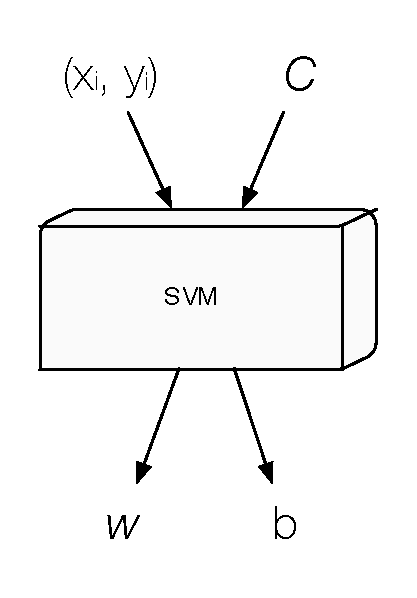
\includegraphics[width=0.25\textwidth]{figuras/svm-extracaowb.eps}
    \caption{Cálculo de $w$ e $b$ a partir dos descritores e $C$}
  \end{center}
\end{figure}

Para inserir os descritores no LIBSVM, junto com os parâmetros, e treinar o classificador são utilizados os métodos \textit{Libsvm::Problem\#set\_examples} e \textit{Libsvm::Model.train}. O primeiro recebe apenas os descritores e os une na estrutura interna da biblioteca, mostrado na linha 4 do código a seguir, e o segundo recebe esses dados em conjunto com os parâmetros, mostrado na linha 5 do código:

\begin{lstlisting}
  class Classificador
    # (...)
    def definir_modelo
      @problema.set_examples(@treinador.classes, @treinador.vetores_de_treino)
      @modelo = Libsvm::Model.train(@problema, @parametro)
    end
    # (...)
  end
\end{lstlisting}

Nesse momento, através do método \textit{Libsvm::Model.train}, $w$ e $b$ já estão definidos e armazenados na instância do modelo. O SVM já está com as informações disponíveis para classificar futuras ocorrências, porém resta apenas saber se o mesmo possui uma boa taxa de acerto ou não. 

Para elevar a taxa de acerto do classificador, o mesmo é treinado e testado com diversos valores para o parâmetro $C$, utilizando o mesmo conjunto de descritores. A finalidade é encontrar valores de $w$ e $b$ que retornem as classes ${y}_{i}$ dos vetores de características ${x}_{i}$ mais próximas da realidade. Os resultados da fase de teste para os valores do parâmetro $C$ escolhidos são exibidos na Tabela 5.3.

Para propriamente implementação da fase teste do classificador é a mesma que propriamente o processo de classificação, por isso os dois processos são explicados de forma única na seção seguinte.

\subsection*{Classificação e teste}

Ambas fases de teste e classificação utilizam o mesmo código, se diferenciando apenas pelo conjunto de publicações que carregados. Para carregar as publicações é utilizado o mesmo processo feito entre as linhas 4 e 8 do Código 5.1.

Para propriamente classificar as publicações, ou seja, obter suas classes, é utilizado o método \textit{Libsvm::Problem\#predict}. Como o modelo instanciado já resolveu a Equação 4.1 de acordo com os dados informados, é possível fazer uma chamada ao método passando uma publicação específica e receber o valor de sua classe.

No processo anterior, o modelo foi alimentado com diversas informações de ${x}_{i}$ e ${y}_{i}$, possibilitando que ele gerasse os valores de $w$ e $b$. Como ambos já estão definidos, agora, é possível introduzir um dado de ${x}_{i}$ (uma publicação) e receber de volta o seu ${y}_{i}$, a sua classe, como definido na Equação 4.2 e na Figura 5.4.

\begin{figure}[htpb]
  \begin{center}
    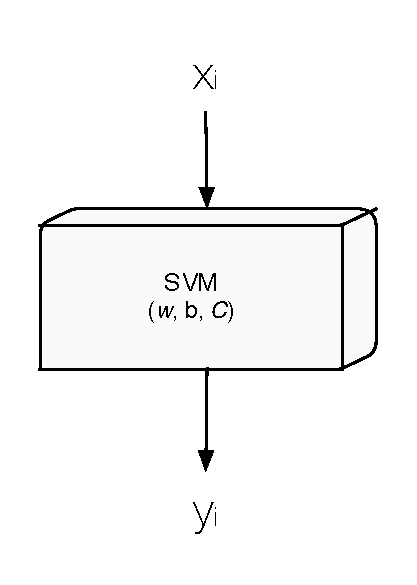
\includegraphics[width=0.25\textwidth]{figuras/svm-testexiyi.eps}
    \caption{Obtenção da classe ${y}_{i}$ através do fornecimento do vetor ${x}_{i}$}
  \end{center}
\end{figure}

Então, ao realizar a chamada para o método \textit{Libsvm::Problem\#predict}, na linha 7 do código a seguir, passando o vetor de uma publicação ${x}_{i}$, é recebida a sua classe ${y}_{i}$ como retorno, com os valores ``1.0'' ou ``-1.0''.

Para registrar a saída das classes, elas são gravadas em um novo arquivo CSV, que contém as informação das publicações e as classes (como é feito manualmente na fase de treino). O código, juntamente ao salvar a classe, também salva a cidade da publicação. No código a seguir, \textit{linha\_csv} representa cada linha do arquivo CSV (uma publicação) no formato de um vetor, até o momento da classificação, cada linha possui 6 posições (da 0 a 5), então as novas informações são adicionadas da sétima posição em diante, como indicado nas linhas 8 e 9 do código a seguir:

\begin{lstlisting}
  class Classificador
    # (...)
    def testar_modelo caminho_saida
      CSV.open(caminho_saida, "w") do |csv|
        @publicacoes.each do |publicacao|
          linha_csv = publicacao.linha_csv
          classe = @modelo.predict(publicacao.vetor)
          linha_csv[6] = classe
          linha_csv[7] = publicacao.cidade
          csv << linha_csv
        end
      end
    end
    # (...)
  end
\end{lstlisting}

Finalmente, para gerar o arquivo CSV final com apenas as publicações positivas - que serão apresentadas no ambiente interativo - são percorridas as publicações e gravados em outro arquivo apenas as que possuem o valor ``1.0'' no campo da sua classificação:

\begin{lstlisting}
  class Classificador
    def filtrar_arquivo_de_classificacoes_positivas caminho_entrada, caminho_saida
      CSV.open(caminho_entrada) do |csv_entrada|
        CSV.open(caminho_saida, 'w') do |csv_saida|
          csv_entrada.each do |linha_entrada|
            csv_saida << linha_entrada if linha_entrada[6] == "1.0"
          end
        end
      end
    end
  end
\end{lstlisting}

\section{Resultados}

Foram obtidas 30.198 publicações do Twitter que contém a palavra-chave ``manifestação'', referentes ao mês de agosto de 2014. Desse conjunto, foram selecionadas 243 publicações de treino positivas e 233 negativas, totalizando 476 publicações de treino. Para a fase de testes, foram selecionadas 70 positivas e 70 negativas, totalizando 140 publicacões de teste.

\subsection*{Testes}

Para a fase de testes, o SVM foi executado diversas vezes, uma para cada valor para o parâmetro $C$. A Tabela 5.1 indica a taxa de acerto obtida para cada valor de $C$, junto com o tempo que necessário para a classificação.

\begin{table}[ht]
  \caption{Taxa de acerto SVM.}
  \centering
  \begin{tabular}{| c | c | c |}
    \hline
    \textbf{$C$} & \textbf{Taxa de acerto} & \textbf{Performance} \\ [0.5ex] \hline \hline
    ... & 50\% & ... \\ \hline
    0.001 & 50\% & 9,4s \\ \hline
    0.01 & 78,5\% & 9,3s \\ \hline
    0.1 & 90,5\% & 8,0s \\ \hline
    1 & 89.5\% & 7,9s \\ \hline
    10 & 86.5\% & 7,6s \\ \hline
    100 & 86.5\% & 7,8s \\ \hline
    1000 & 86.5\% & 7,5s \\ \hline
    ... & 86.5\% & ... \\ [1ex]
    \hline
  \end{tabular}
  \label{table:nonlin}
\end{table}

Foi percebido, que para um valor muito baixo de $C$, o classificador adquire o comportamento de classificar todas as publicações como positivas. Já para um valor muito alto de $C$, a taxa de acerto se manteve em 86,5\%. O valor otimizado para $C$ foi encontrado para o valor ``0.1'', no qual o classificador exibiu a maior taxa de acerto, de 90,5\%. A performance, apesar de variar, não se mostrou muito relevante para o modelo.

\subsection*{Total de publicações e localização}

Após a classificação, as publicações positivas somaram 13.611 e as negativas 16.587. 

As publicações positivas e negativas exibem divergência no que diz respeito a extração da cidade e geolocalização. As positivas exibiram maior possibilidade de extração da sua cidade, através do texto da publicação ou do perfil do usuário. Já as negativas, exibiram quase 3 vezes mais o dado de geolocalização, apesar de ainda ser em baixa quantidade (3.6\%).

Ainda nas publicações positivas, para os dados de localização contidos na publicação ou no perfil do usuário, foi possível a extração da informação em 8.148 publicacões (60\% delas). A Tabela 5.3 indica os resultados para os dados extraídos:

\begin{table}[ht]
  \caption{Resultados da classificação e dos dados extraídos.}
  \centering
  \begin{tabular}{| c || c | c | c |}
    \hline
    \textbf{Publicações} & \textbf{Quantidade} &  \textbf{Com cidade} & \textbf{Com geolocalização} \\ [0.5ex] \hline \hline
    \textbf{Positivas} & 13.611 & 8148 (60\%) & 177 (1.3\%) \\ \hline
    \textbf{Negativas} & 16.587 & 8700 (52.4\%) & 610 (3.6\%) \\ \hline
    \textbf{Total} & 30.198 & 16.848 (56\%) & 787 (1.9\%) \\ [1ex]
    \hline
  \end{tabular}
  \label{table:nonlin}
\end{table}

Das publicações positivas, apenas 177 delas (cerca de 1\%) contem a geolocalização. Isso demonstra que a grande maioria das publicações ainda está sendo enviada pelo computador ou por dispositivos sem o GPS ativado.

\subsection{Análise visual e ambiente}

Segundo \citeonline{Thomas2005}, \textit{Análise Visual} é ``a ciência do raciocínio analítico facilitada por interfaces visuais interativas''. A área tem recebido crescente atenção por conta do processo de \textit{Big Data}, aonde é estudado como processar grandes volumes de informações, de modo que possam ser geradas análises em cima das mesmas. Como apontam \citeonline{Zhicheng2013} e \citeonline{Begoli2012}, uma das formas de análise é a visual, aonde, torna-se possível tirar conclusões através do raciocínio permitido por meio da visão e da organização de informações favoráveis a isso. 

No ambiente interativo, criado a partir do modelo implementado, é possível analisar visualmente o comportamento das publicações segundo o seu horário e localização. É possível enxergar a existência de picos de publicações em determinados horários, o que podem indicar eventos, e de onde estão surgindo essas publicações, para examinar a localização de cada evento.

Para analisar os eventos, no ambiente interativo (disponível em: \url{http://deteccao.zangrandi.me/}) são exibidos gráficos de séries-temporais das publicações, criados a partir da ferramenta \textit{Highcharts}\footnote{http://www.highcharts.com}, e mapas de marcadores, criados a partir do \textit{TileMill}\footnote{https://www.mapbox.com/tilemill/}.

\subsubsection*{Análise do horário}

Se houve um grande pico de publicações em uma determinada faixa de horário, a possibilidade é que naquela faixa haja a ococrrência de um ou mais eventos. E quanto maior o pico de publicações, maior a magnitude do evento. Através da taxa de acerto obtida na fase de teste da classificação, é possível dizer que 90\% das publicações dizem respeito ao evento de manifestação que o modelo se propõe a detectar.

O gráfico da Figura 5.5 mostra a frequência de publicações relacionadas à manifestações durante cada dia do mês de agosto:

\begin{figure}[htpb]
  \begin{center}
    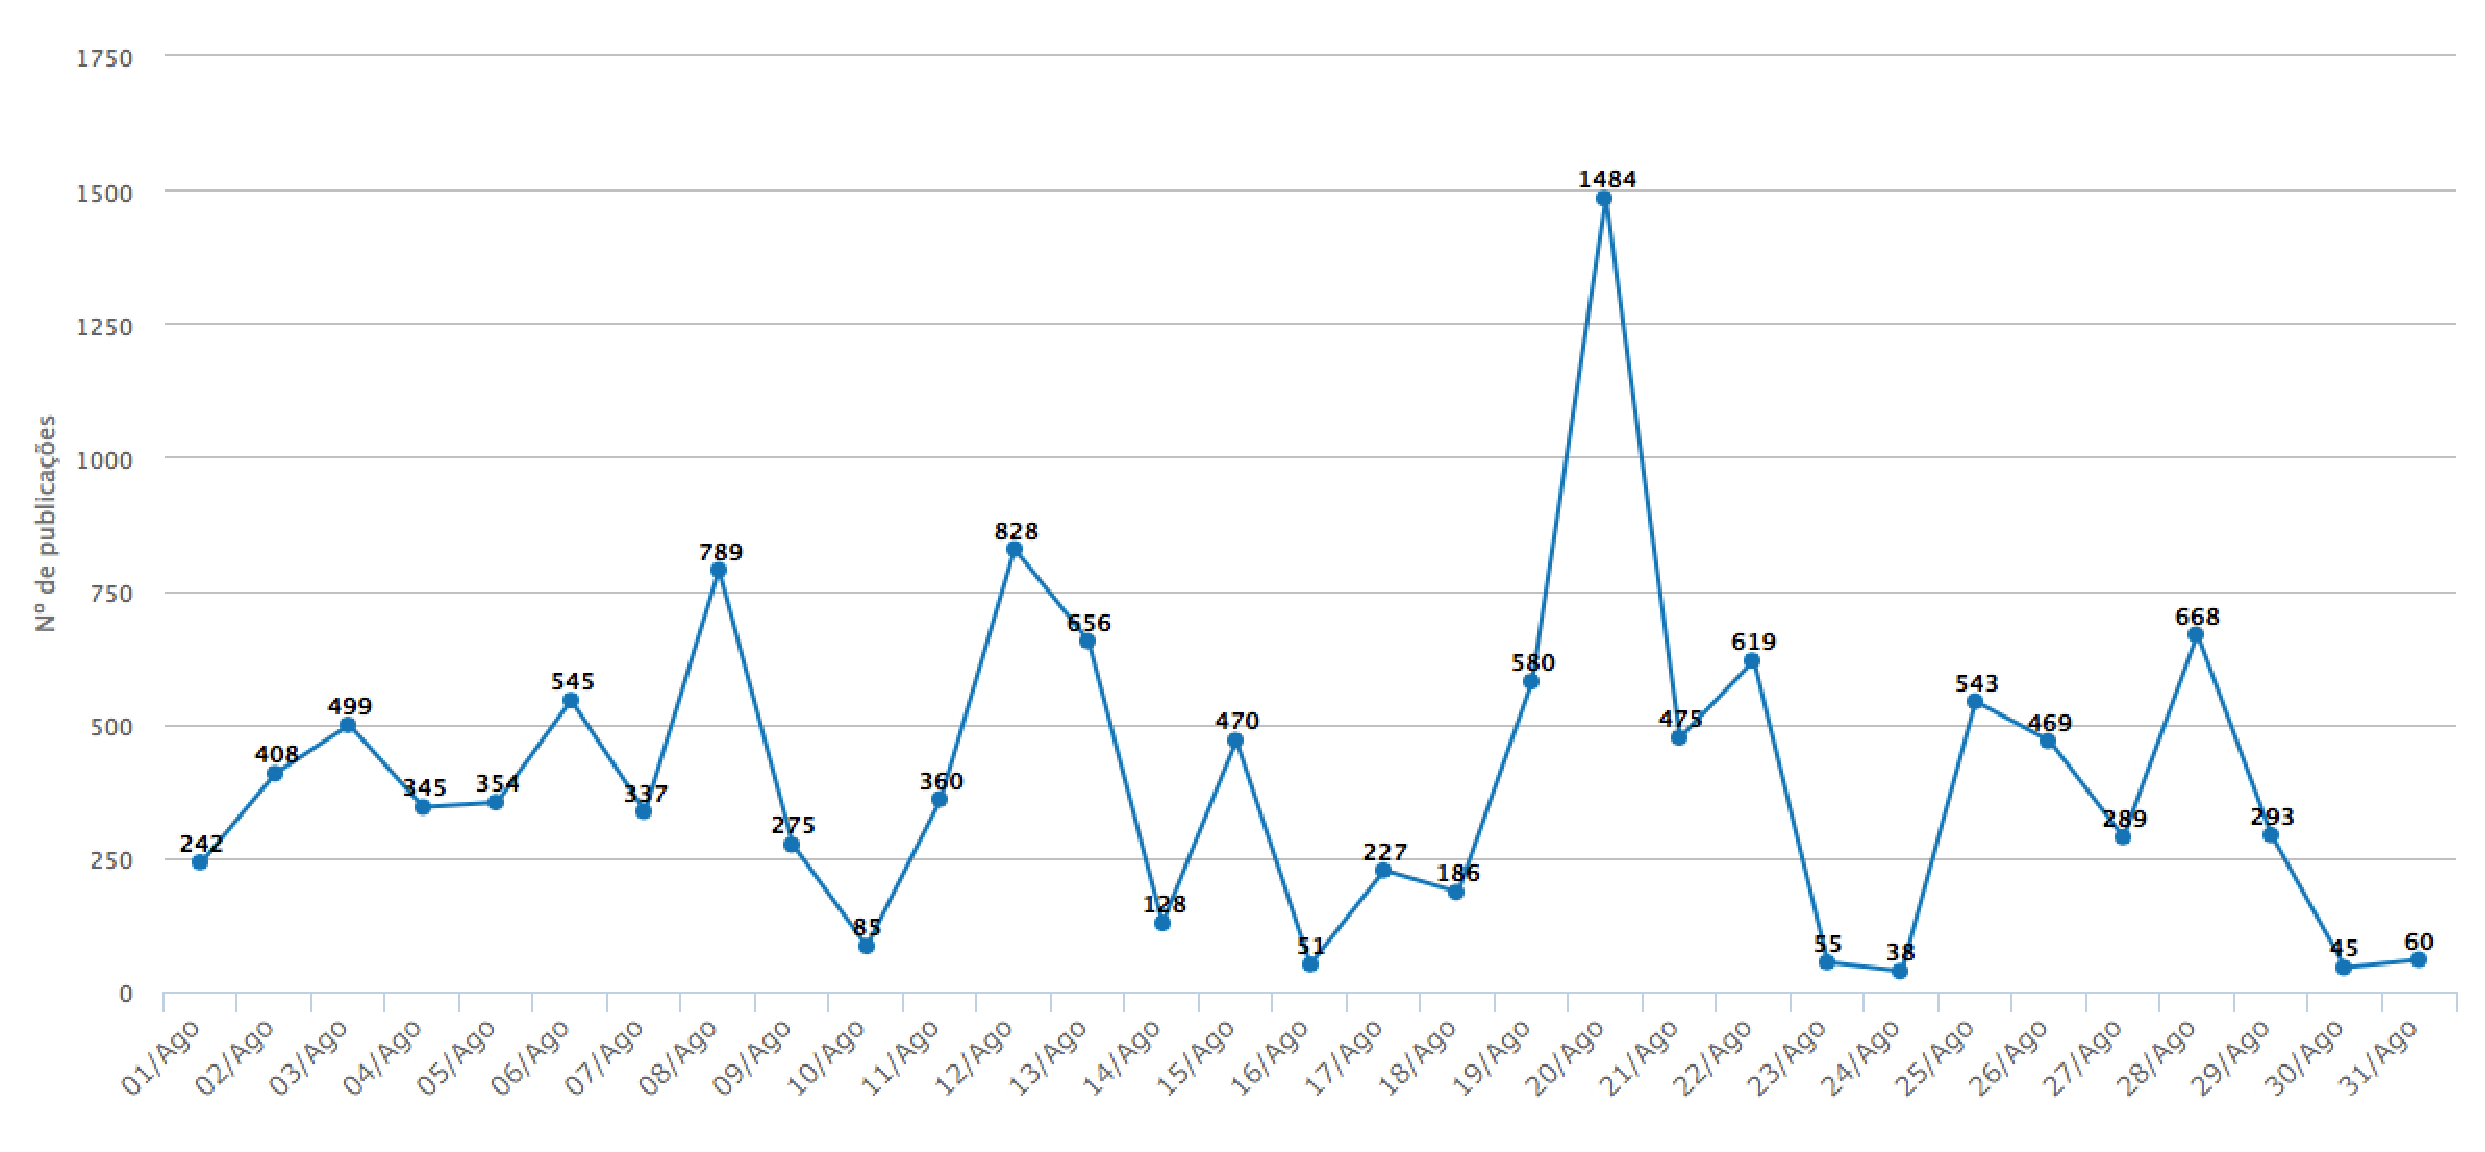
\includegraphics[width=1.0\textwidth]{figuras/grafico-mes.pdf}
    \caption{Publicações do mês de agosto.}
  \end{center}
\end{figure}

É possível observar variações na quantidade de publicações enviadas em cada dia. Particularmente, no dia 20 de agosto, há um grande pico de publicações, podendo indicar algum evento relevante naquele dia. Os dias 08 e 12 também apresentam um número de publicações acima da média. Porém, como o Twitter possui comportamento dinâmico, para chegar à análise dos eventos propostos pelo modelo - manifestações com local e horário - a frequência das publicações devem ser analisadas por dentro de cada dia, por faixa de horário. 

No ambiente interativo, ao clicar em qualquer ponto no gráfico mensal, é exibido o \textit{gráfico diário} daquele dia. Nesse gráfico, também no formato de série-temporal, são apresentadas as publicações por faixa de horário de 1h. Ao analisar as publicações do dia 20 de agosto, por exemplo o seguinte gráfico da Figura 5.6 é apresentado.

\begin{figure}[htpb]
  \begin{center}
    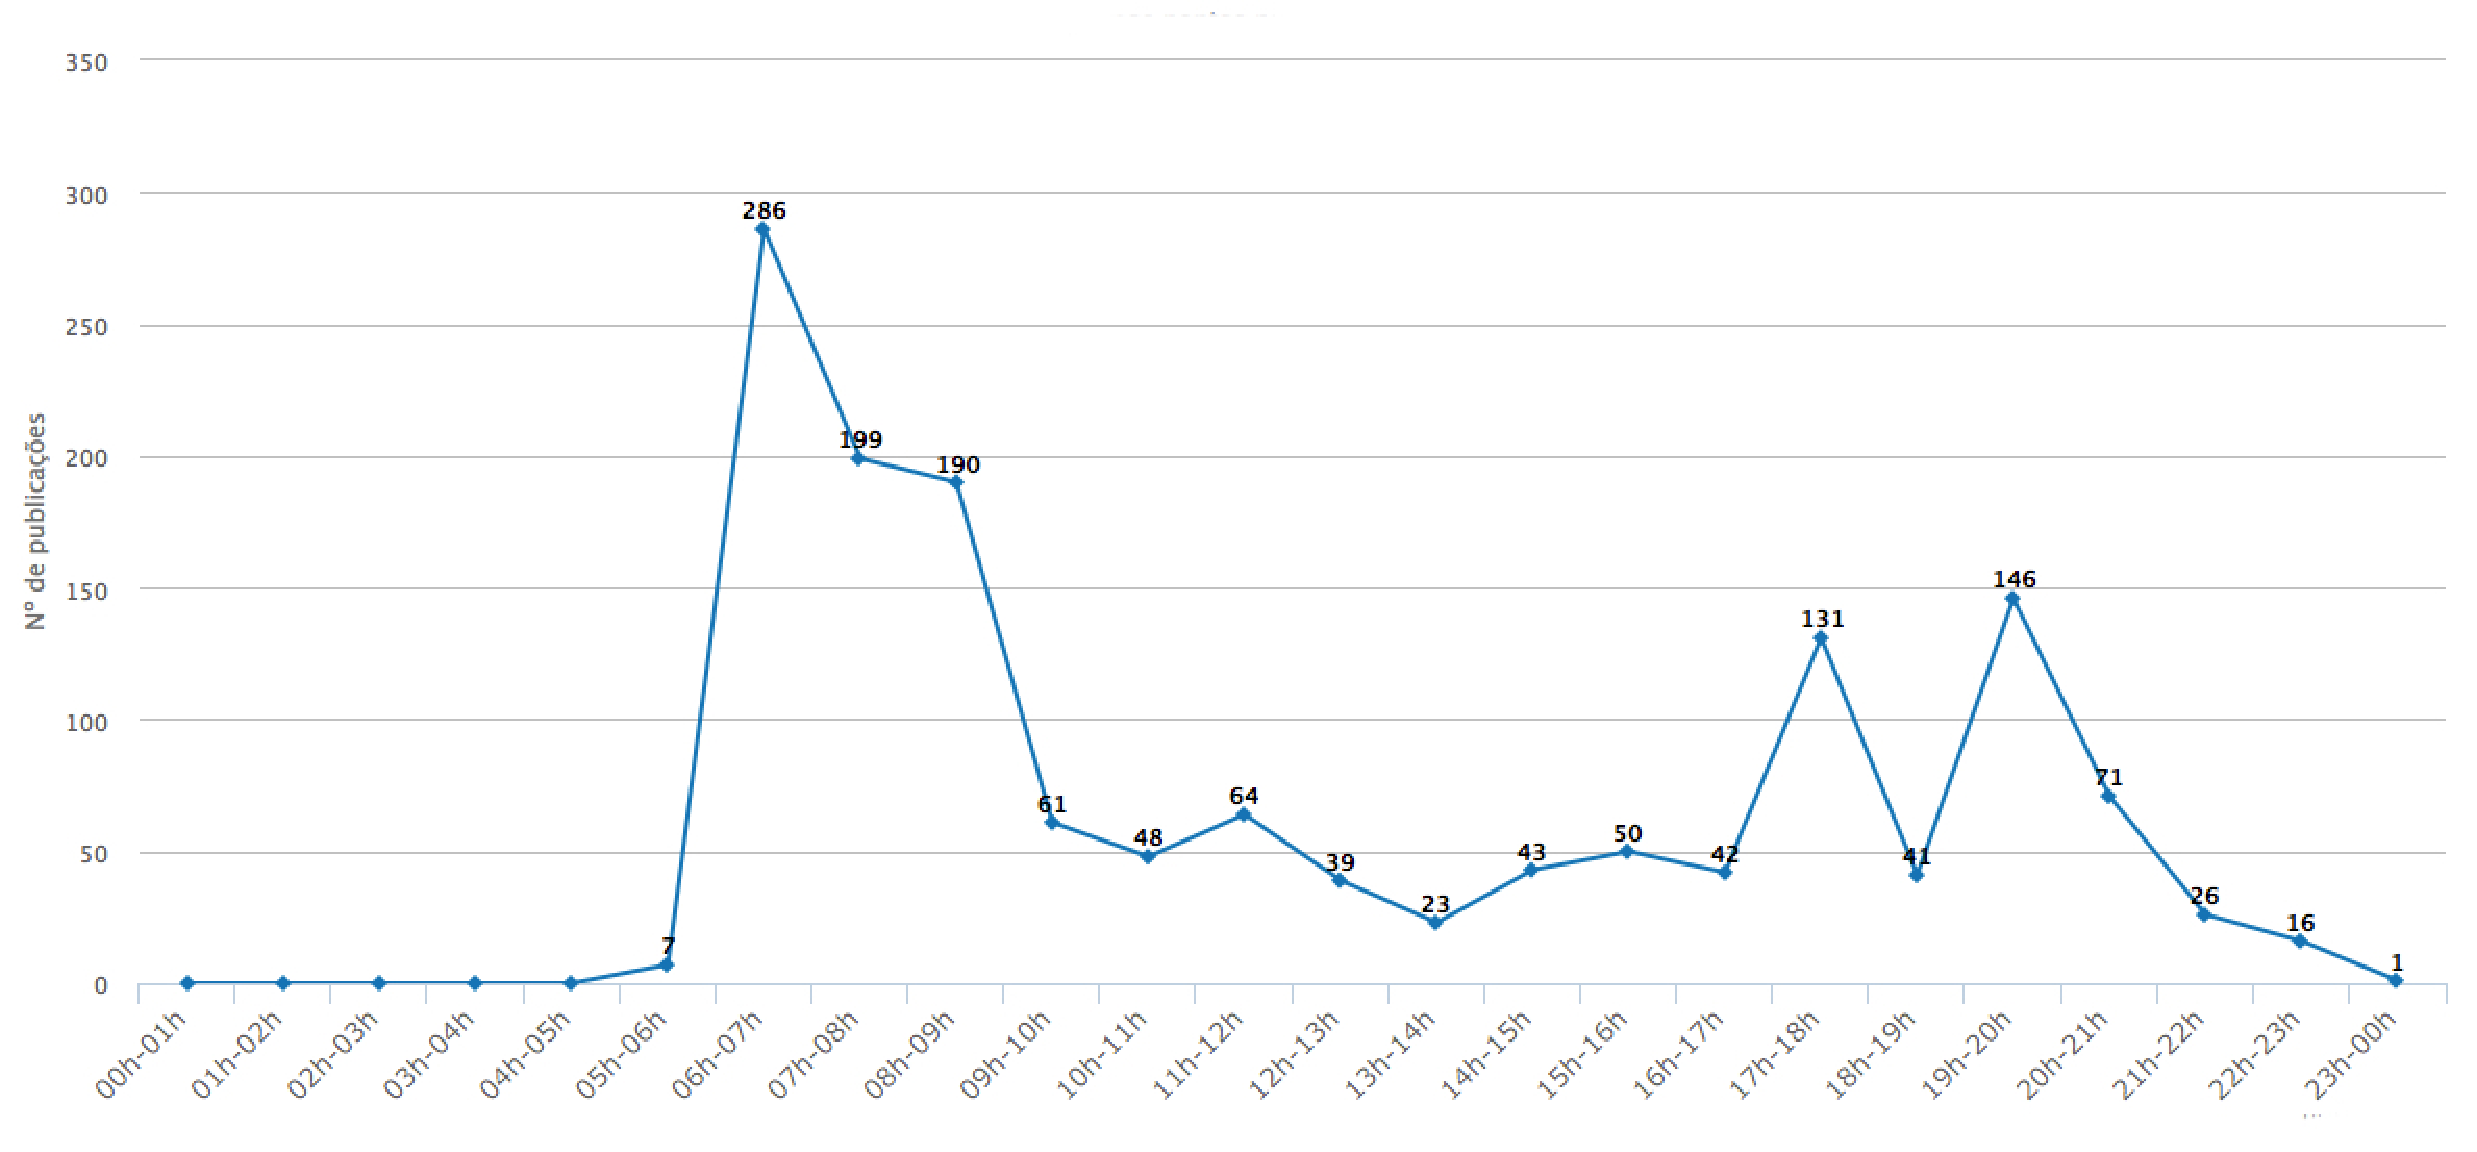
\includegraphics[width=1.0\textwidth]{figuras/grafico-dia.pdf}
    \caption{Publicações do dia 20 de agosto.}
  \end{center}
\end{figure}

No gráfico, é possível visualizar o aparecimento de um grande pico de publicações na faixa de 06h às 07h do dia 20 de agosto. O pico de publicacões reverbera até a faixa de 08h-09h, e novamente ocorrem dois picos nas faixas 17h-18h e 19h-20h.

Com os picos de publicações visíveis e o horário dos eventos aparente, para analisar de onde estão surgindo as publicações e sobre qual evento específico elas estão se referindo, as publicações são exibidas distribuídas no \textit{mapa de marcadores}.

Para o modelo implementado, os vales, ou seja, os pontos de baixa no número de publicações não são relevantes. Em relação ao evento de manifestação, quando não há a sua menção, simplesmente a sua ocorrência não necessita ser detectada. Porém, em aplicações em outros âmbitos como políticos ou comerciais, os vales podem ser interessantes na medida em que determinam uma baixa de popularidade, e talvez seja possível uma ação específica para esse caso.

\subsubsection*{Análise do evento e da localização}

Ao clicar em qualquer ponto do gráfico por faixa de horário, é exibido um mapa de marcadores, no qual é possível visualizar o conteúdo de cada publicação disponível, bem como sua localização exata, para publicações com geolocalização, ou aproximada, para publicações com o registro da cidade. 

As publicações que não contém a geolocalização são aproximadas através do mapeamento das cidades para a sua geolocalização, de acordo com a informação do IBGE\footnote{http://ibge.gov.br/}. O órgão fornece a informação de geolocalização de cada cidade brasileira. A informação serve para marcar corretamente a cidade no mapa apresentado.

Cada mapa de marcador pode exibir os seguintes objetos:

\begin{itemize}
  \item \textbf{Marcador azul escuro:} Publicação única com localização exata.
  \item \textbf{Marcador azul claro:} Publicação única com localização aproximada.
  \item \textbf{Círculo verde:} Pequeno agrupamento de publicações (entre 2 e 10).
  \item \textbf{Círculo amarelo:} Médio agrupamento de publicações (entre 10 e 100).
  \item \textbf{Círculo vermelho:} Grande agrupamento de publicações (maior do que 100).
\end{itemize}

Ao clicar no ponto das publicações entre as 06h e 07h do dia 20 de agosto o mapa da Figura 5.7 é exibido:

\begin{figure}[h!]
  \begin{center}
  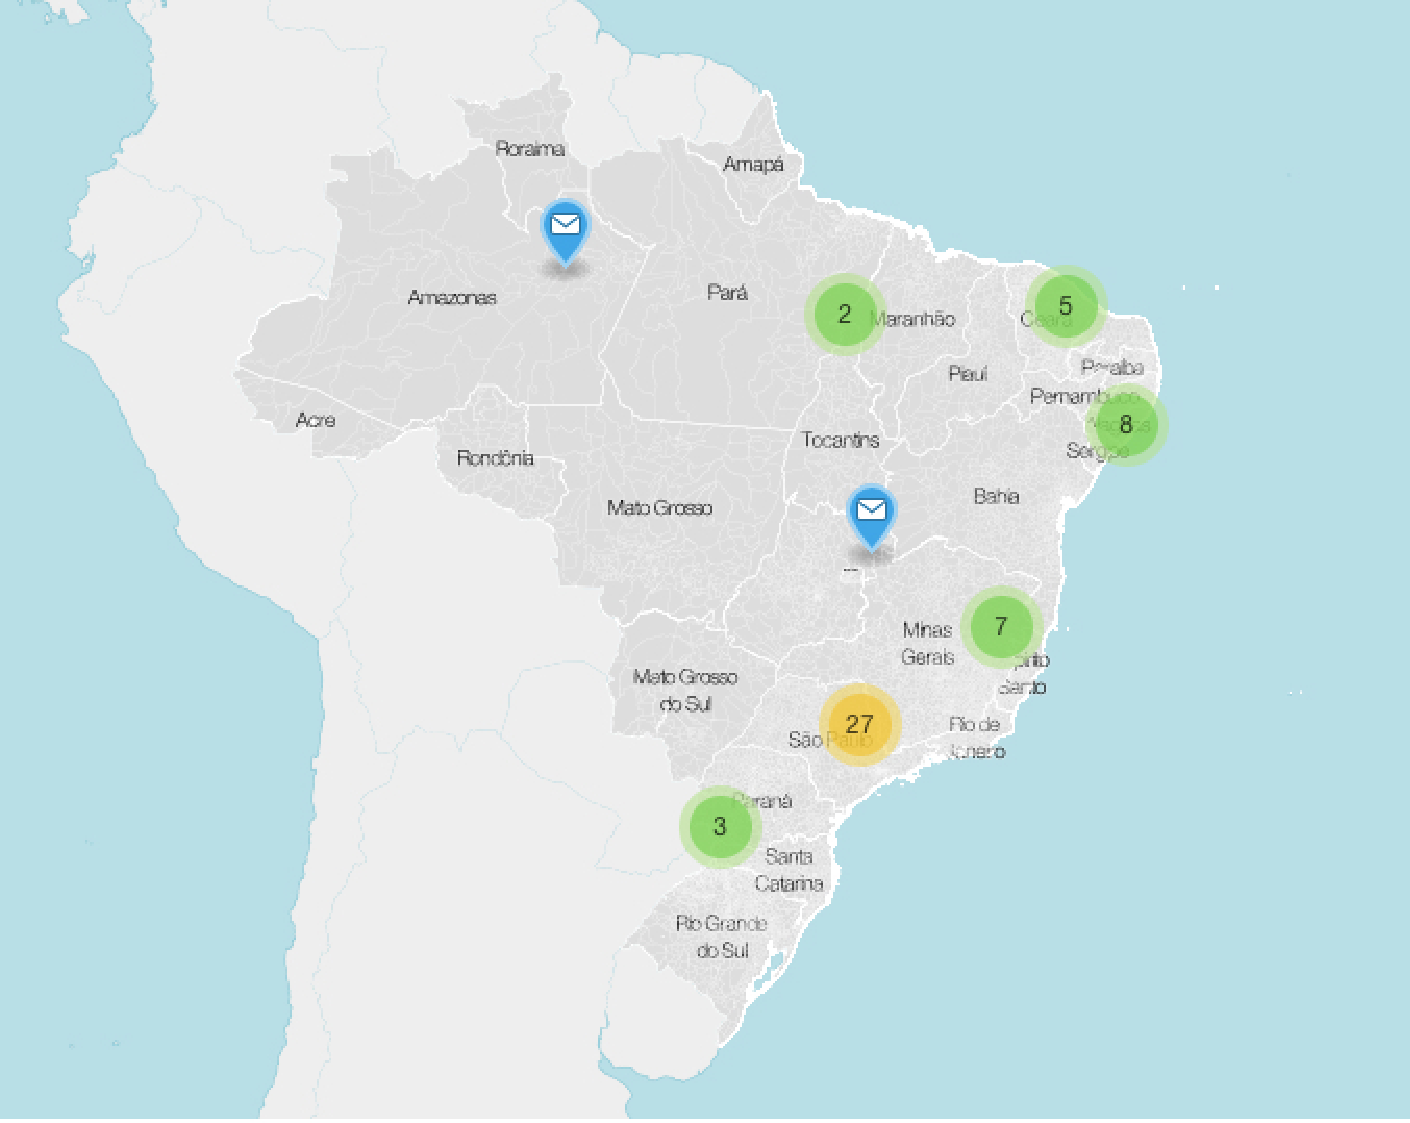
\includegraphics[width=0.8\textwidth]{figuras/mapa-marcador.pdf}
  \caption{Mapa de marcadores para o horário entre 06h e 07h do dia 20/08.}
  \end{center}
\end{figure}

É possível visualizar uma maior concentração de publicações vindas de determinada área do estado São Paulo. Ao aplicar zoom no mapa, o agrupamento de publicações se desfaz, permitindo que as publicacões sejam visualizadas de modo agrupado com mais exatidão, ou também de modo único. 

Ao ampliar o mapa no sentido dessa concentração, o mapa da Figura 5.8 é exibido.

\begin{figure}[h!]
  \begin{center}
  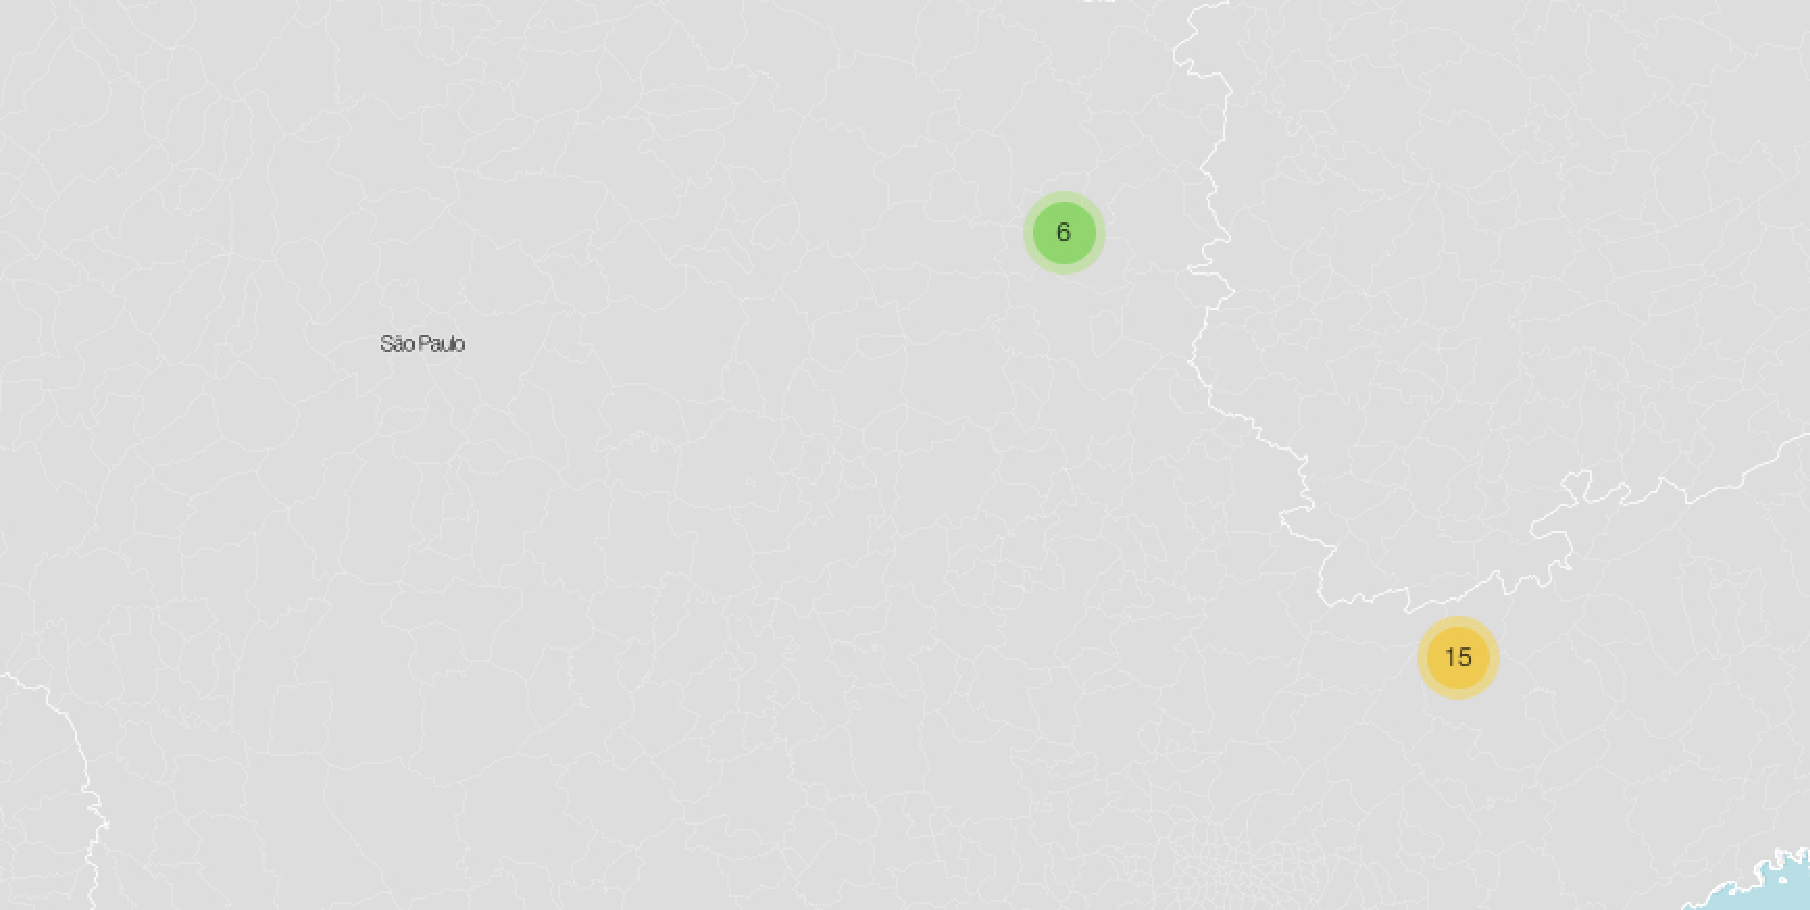
\includegraphics[width=1.0\textwidth]{figuras/mapa-marcador-2.pdf}
  \caption{Concentração de publicações em São Paulo.}
  \end{center}
\end{figure}

Antes, as 27 publicações que agrupadas em determinada área, através da ampliação do mapa se diviram em áreas menores, sendo as maiores delas 15 publicações e outra com 6 publicações. Tal informação indica dois polos distintos de surgimento de publicações, o que pode indicar a ocorrência de dois eventos distintos ou não.

Ao amplificar mais uma vez o mapa, já é possível visualizar as publicações de forma única, como indica a Figura 5.9.

\begin{figure}[h!]
  \begin{center}
  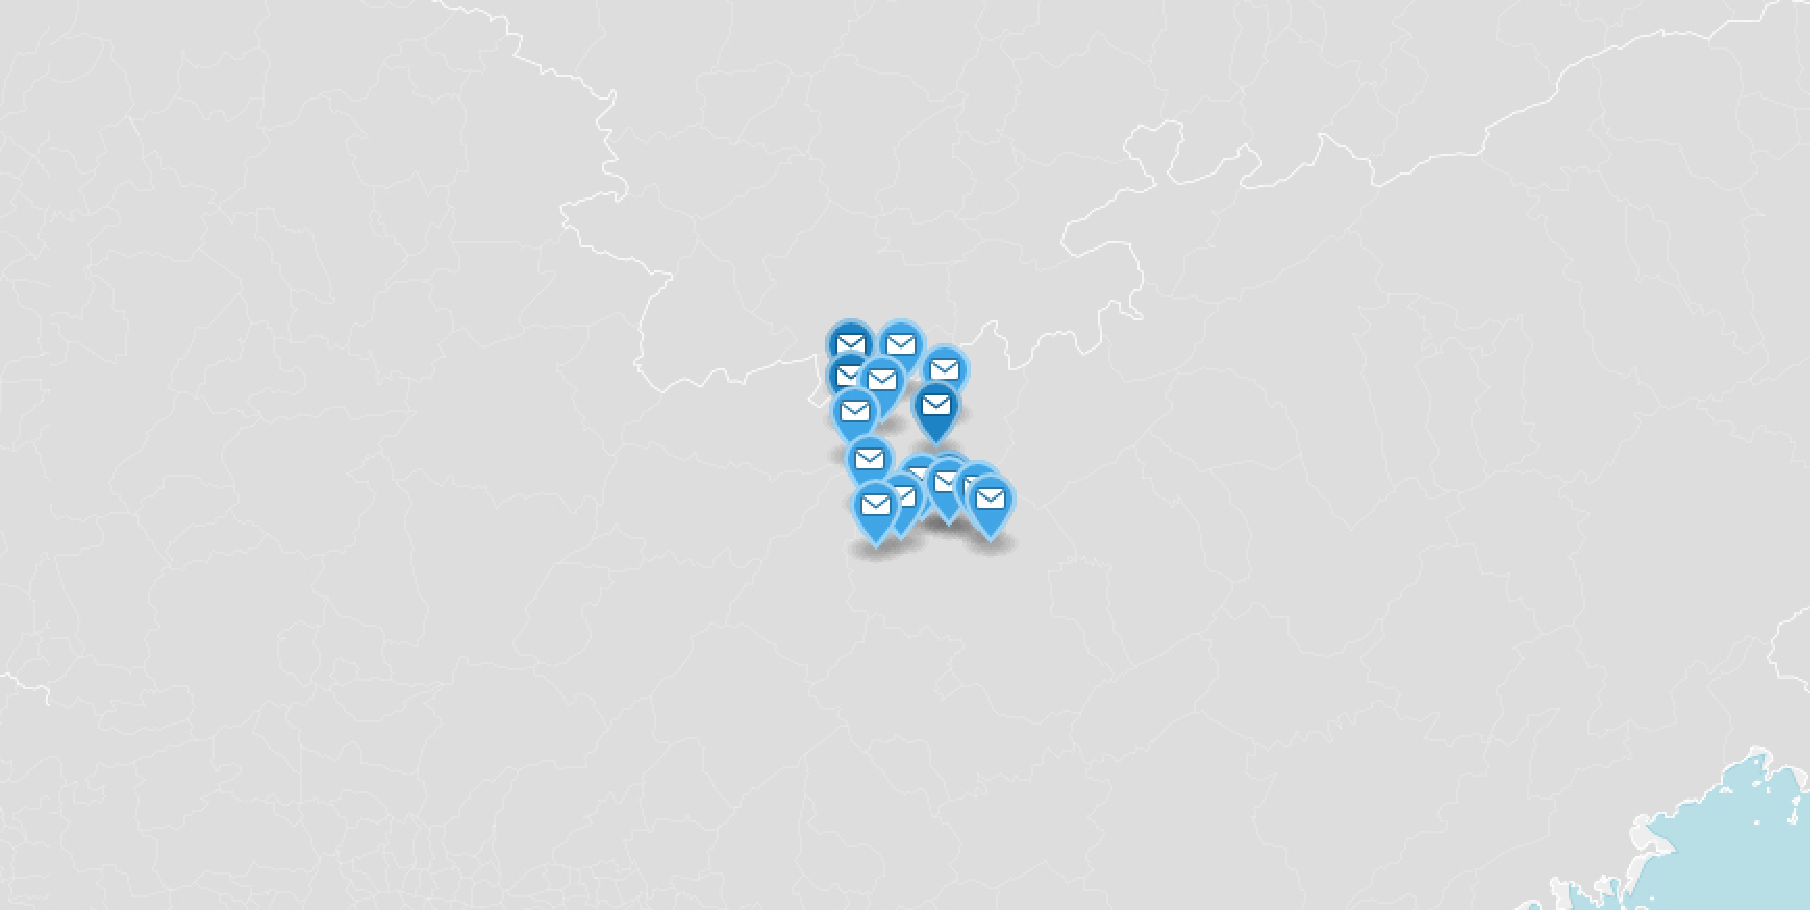
\includegraphics[width=1.0\textwidth]{figuras/mapa-marcador-3.pdf}
  \caption{Publicações únicas em São Paulo.}
  \end{center}
\end{figure}

É possível perceber que, nesse horário, um grande número de publicações está surgindo dessa região de São Paulo. Para obter detalhes e descobrir ao que se refere essa concentração de publicações repentina em determinada localização, é possível clicar em cada marcador e exibir a sua mensagem, como indica a Figura 5.10.

\begin{figure}[h!]
  \begin{center}
  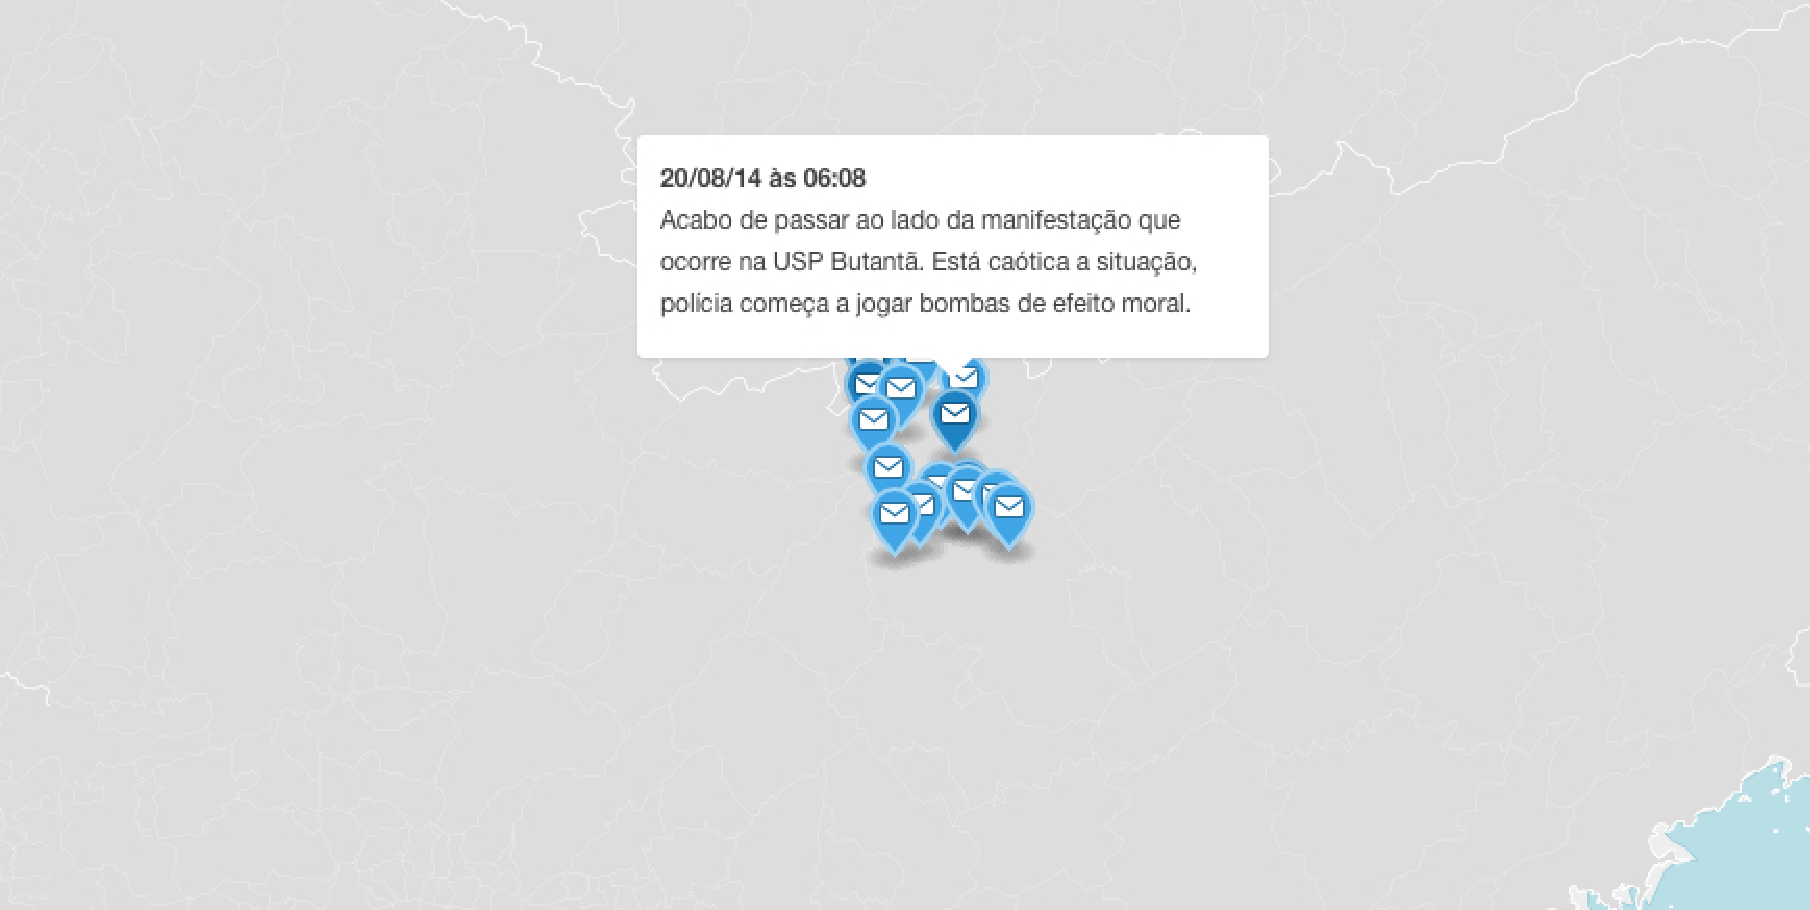
\includegraphics[width=1.0\textwidth]{figuras/mapa-marcador-4.pdf}
  \caption{Agrupamentos de publicações em Minas Gerais e São Paulo.}
  \end{center}
\end{figure}

Através da mensagem da publicação, é possível identificar sobre qual evento a concentração se refere. Nesse caso, o evento em questão foi a ocorrência de uma manifestação no campos da USP Butantã (Universidade de São Paulo), o que gerou a erupção de publicações naquela localização e horário.

Há ainda, os picos de publicações das faixas 17h-18h e 19h-20h do dia 20 de agosto, apresentados na Figura 5.4. A faixa entre 17h e 18h exibe grande concentração do estado de Minas Gerais e uma menor concentração em São Paulo, como indica a Figura 5.11. 

\begin{figure}[h!]
  \begin{center}
  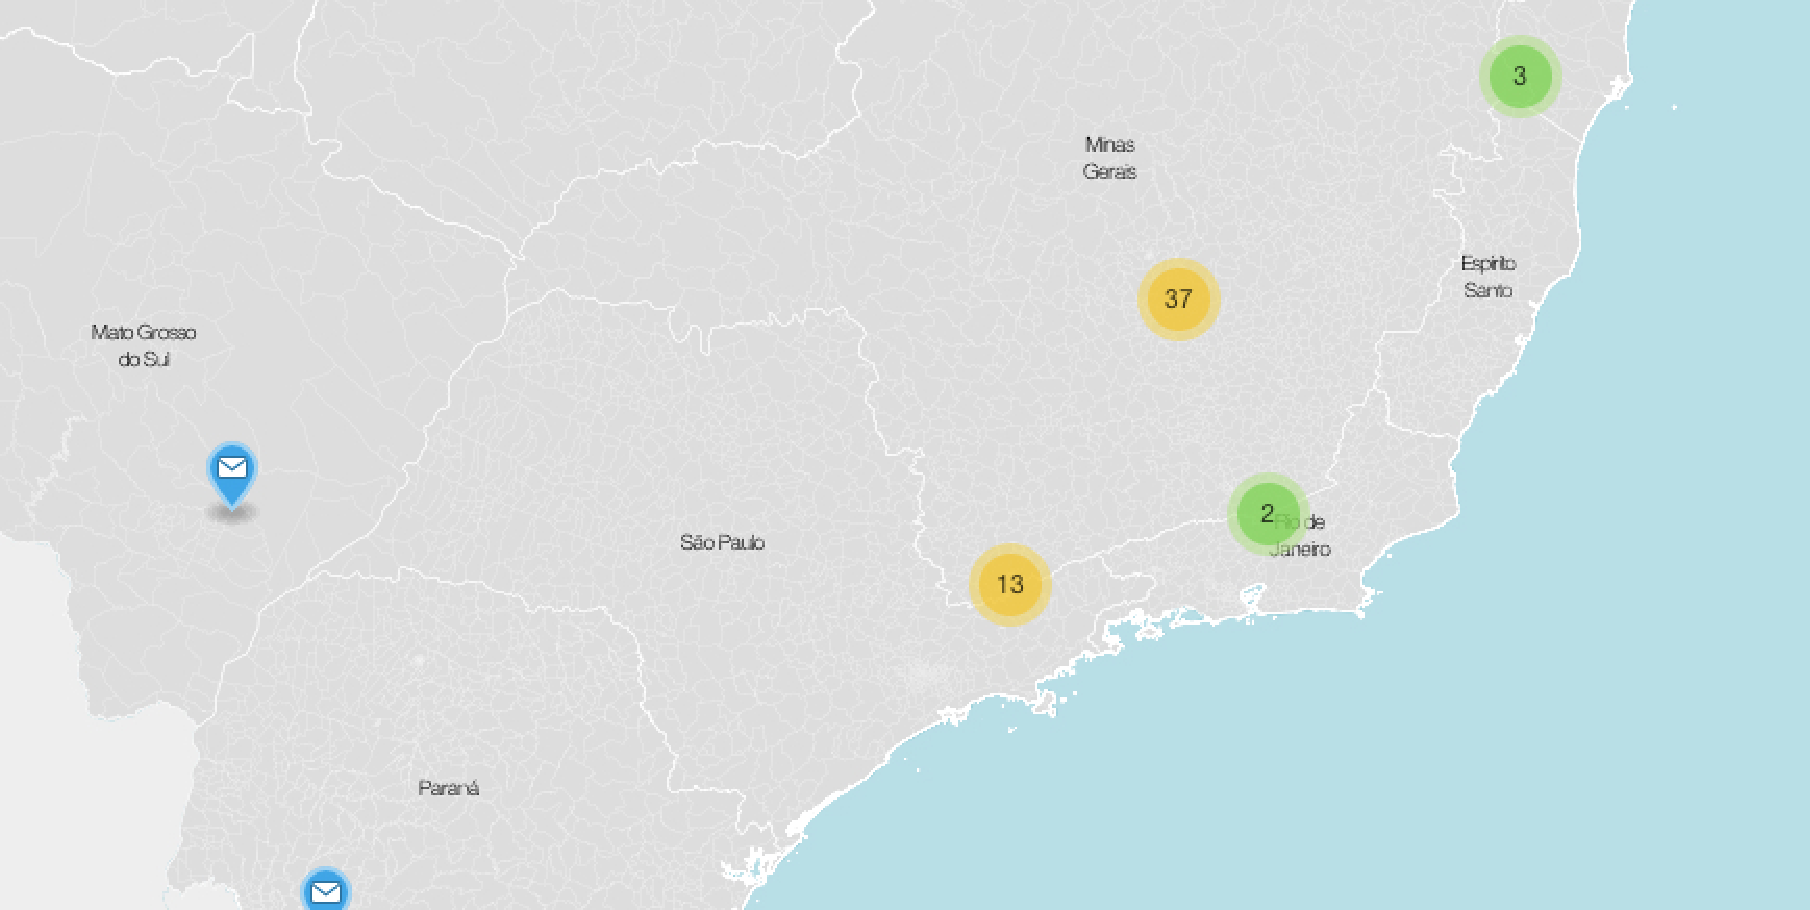
\includegraphics[width=1.0\textwidth]{figuras/mapa-marcador-6.pdf}
  \caption{Mensagem de uma publicação.}
  \end{center}
\end{figure}

Ao ampliar o mapa, é possível identificar dois eventos nessa faixa de horário: uma manifestação que interditou a rodovia MG-040 por volta das 17h40, e outra em frente ao Masp, na Avenida Paulista. Como indicam a Figura 5.12 e 5.13:

\begin{figure}[h!]
  \begin{center}
  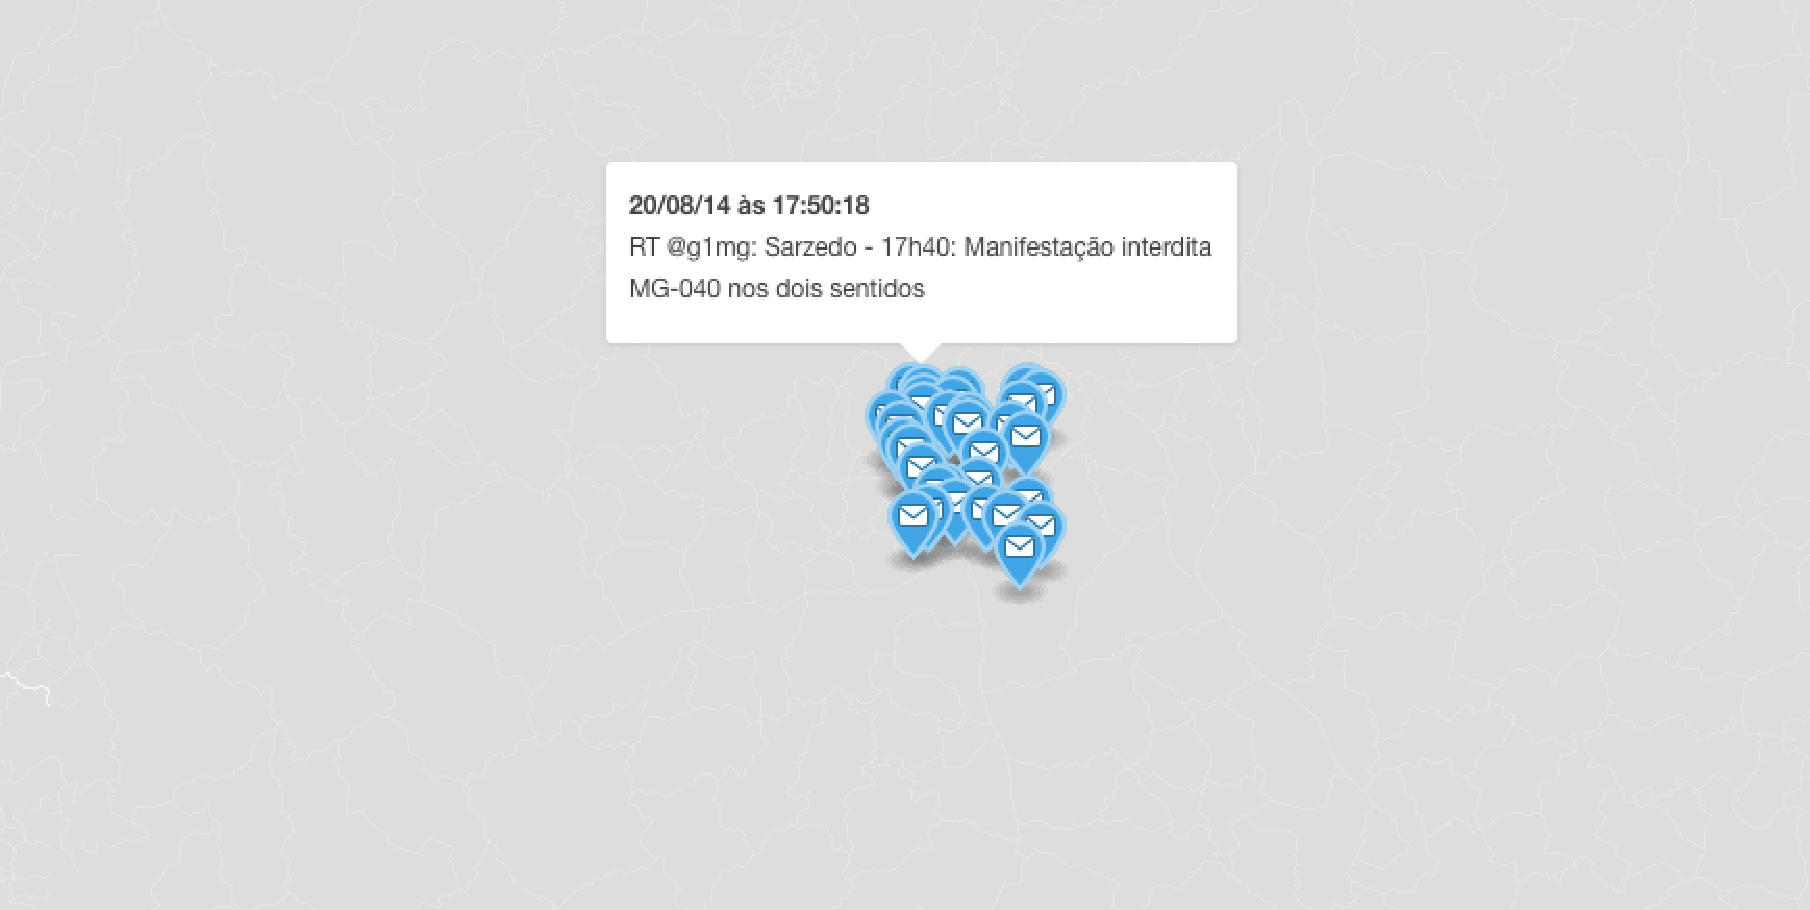
\includegraphics[width=1.0\textwidth]{figuras/mapa-marcador-5.pdf}
  \caption{Manifestação na rodovia MG-040, em Minas Gerais.}
  \end{center}
\end{figure}

\begin{figure}[h!]
  \begin{center}
  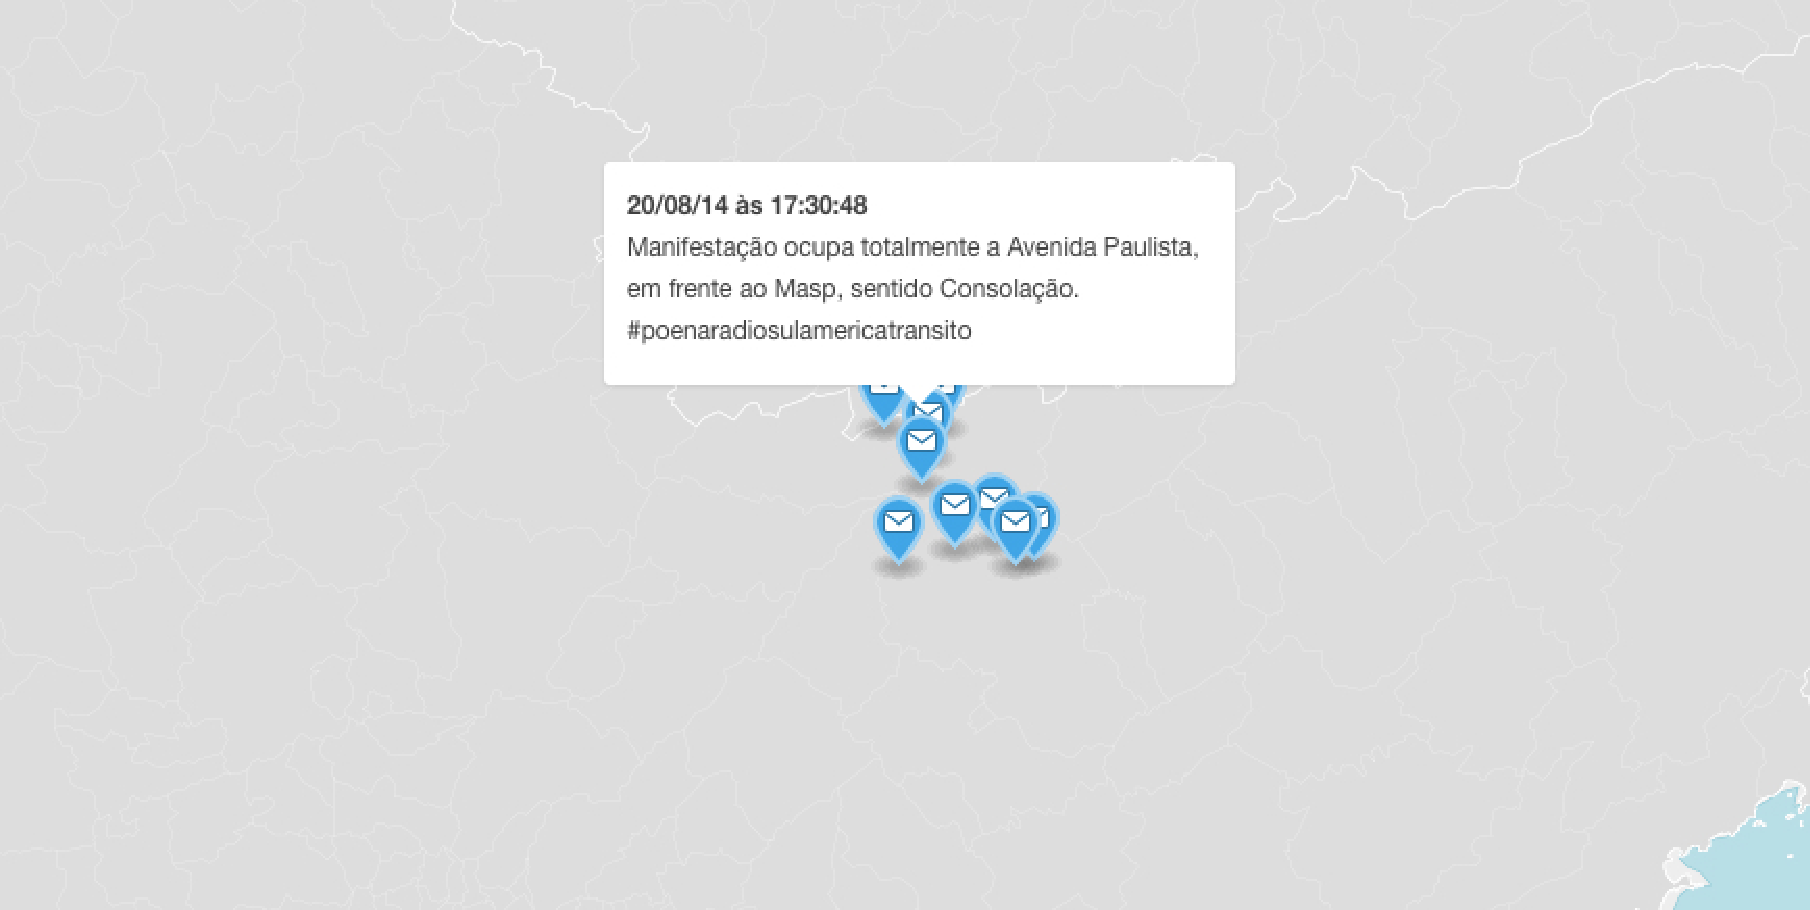
\includegraphics[width=1.0\textwidth]{figuras/mapa-marcador-7.pdf}
  \caption{Manifestação na Avenida Paulista, em São Paulo.}
  \end{center}
\end{figure}

A análise desse dia em específico mostra que o modelo, através de dados esparsos e desordenados em formato de texto, organiza essas informações e as apresenta em um ambiente que permite a análise visual de informações relevantes como o evento ocrrido, a localização aproximada e o seu horário.

% \subsection*{Análise da frequência de termos}

% Para visualizar a frequência dos termos contidos nas publicações de manifestações, é criada uma nuvem de termos, a partir da ferramente JQCloud\footnote{https://github.com/lucaong/jQCloud}. São inseridas as palavras e a sua frequência e a ferramenta gera uma nuvem com os termos mais frequentes em escala maior e vice-versa. Na Figura 5.5 está exibida a nuvem de termos gerada:

% \begin{figure}[h!]
%   \begin{center}
%   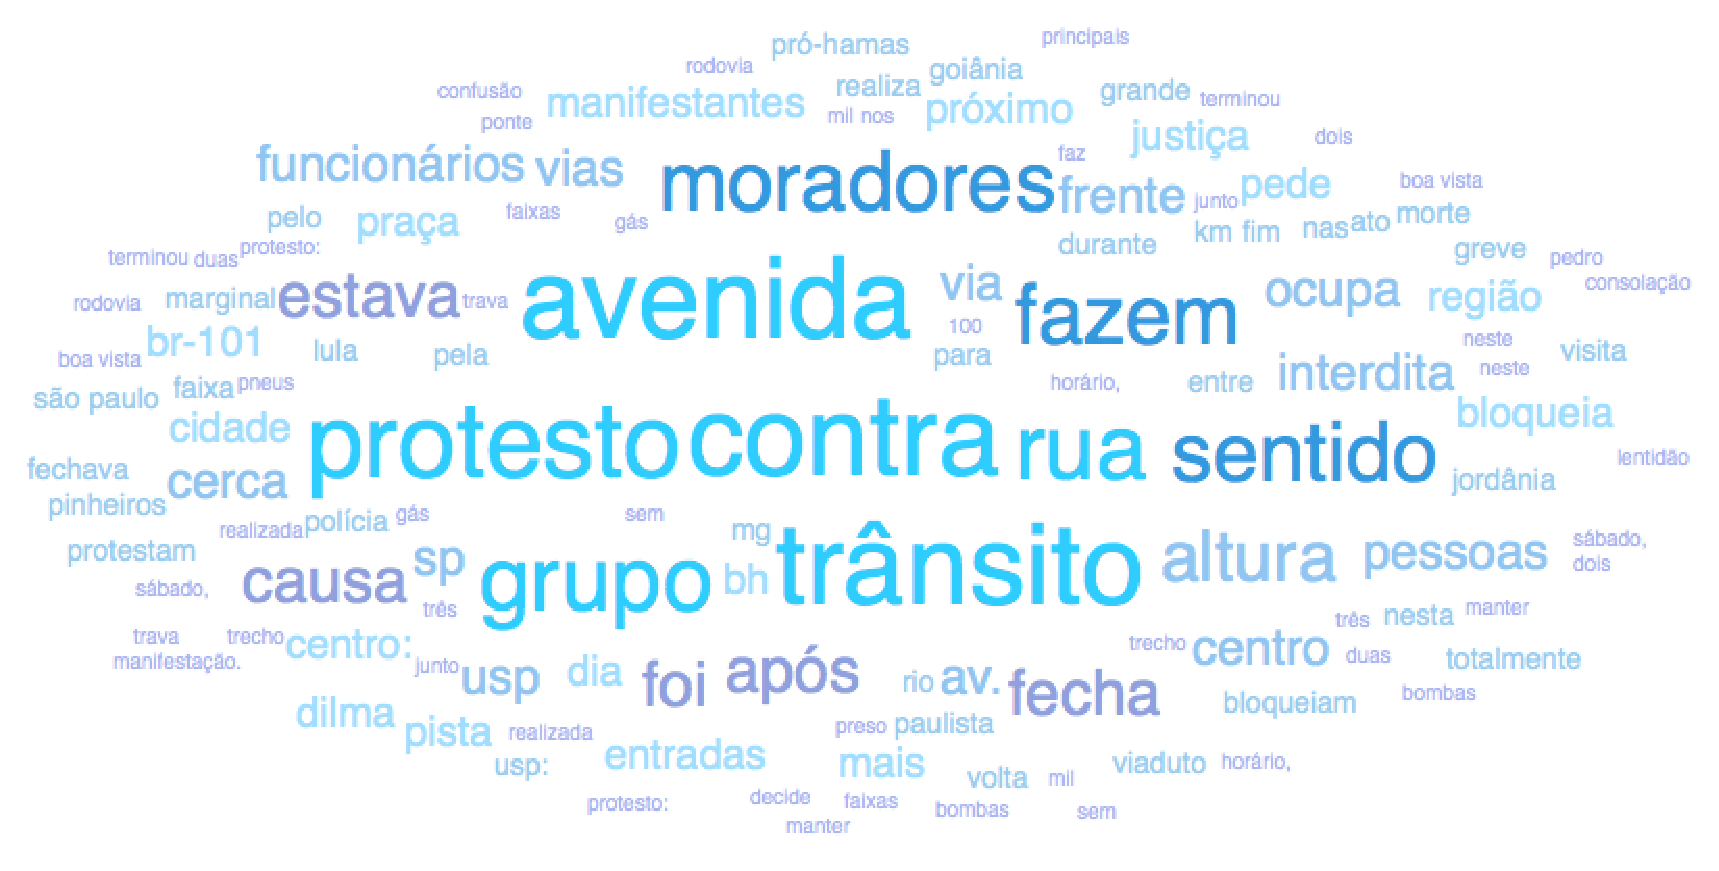
\includegraphics[width=1.0\textwidth]{figuras/nuvem-palavras.pdf}
%   \caption{Nuvem de palavras mais recorrentes.}
%   \end{center}
% \end{figure}

% É possível ver que os termos ``contra'', ``trânsito'', ``avenida'', ``protesto'' e ``grupo'' foram as mais recorrentes nas publicações de manifestações, o que reflete a realidade conhecida. Eventos de manifestações geralmente estão ligados à interdição de avenidas e do trânsito, e são criadas por grupos, contra um determinado objeto.